\section{'t Hooft 算符与赫克修正}
\label{thooftheckeop}

\subsection{本征膜}

本文余下部分的主要目标，是比文献 \cite{KW} 中的阐述更深入地描述 't Hooft 算符与赫克修正\index{hecke-modification@赫克修正}的性质. 我们先作一个简短的介绍，更详细的内容请读者查阅文献 \cite{KW}.

从四维出发，可以用两种方式对 $\N=4$ 超杨--米尔斯理论作扭曲，得到两个拓扑场论（如脚注 \ref{partial} 所述，是部分拓扑的），我们将它们称为 $A$-模型和 $B$-模型. 每个模型都具有半 BPS 线算符\index{line-operator@线算符}，即 $B$-模型中的威尔逊算符和 $A$-模型中的 't Hooft 算符. 下一步是在黎曼曲面 $C$ 上紧化到二维. 支撑在点 $p\in C$ 处的四维线算符，降为二维的线算符.



\begin{figure}[!tp]
\begin{center}
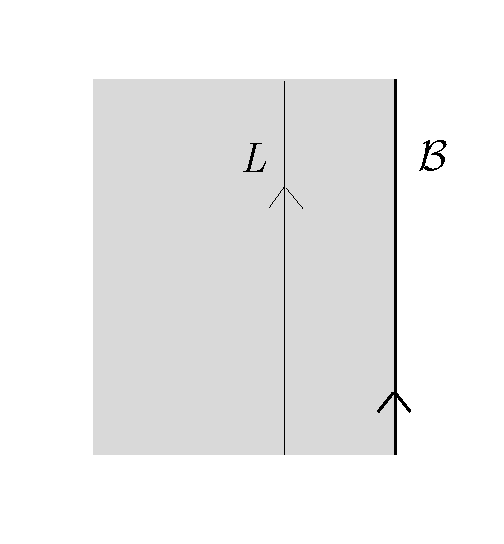
\includegraphics[width=3.5in]{gla8-1.pdf}
\end{center}
\caption{线算符 $L$ 接近由膜 $\B$ 标记的边界. 这给出一个新的复合边界条件\index{boundary-condition@边界条件} $\B'=L\cdot \B$.\label{nuxto}}
\end{figure}

\begin{figure}[!tp]
\begin{center}
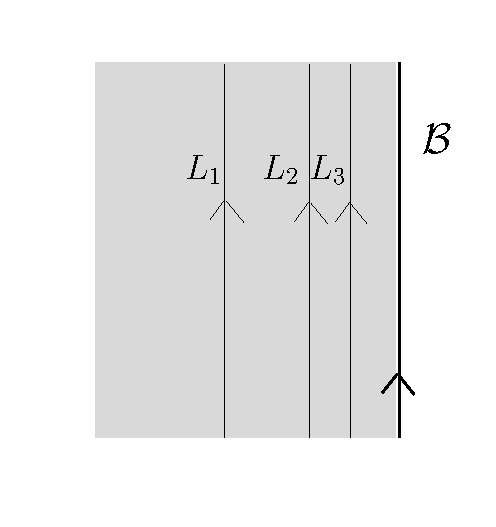
\includegraphics[width=3.5in]{gla8-2.pdf}
\end{center}
\caption{可以将线算符逐个移到边界. 这给出了线算符在膜上的结合性作用. \label{buxto}}
\end{figure}

我们在带边界的二维流形 $\Sigma$ 上研究紧化所得的有效二维理论. 边界条件由膜 $\B$ 定义.（我们将用相同的记号表示膜 $\B$ 和相应的边界条件.）现在的关键是考察线算符接近边界时的行为（图 \ref{nuxto}）. 显然，在二维拓扑场论中，线算符 $L$ 接近具有边界条件 $\B$ 的边界，会产生一个新的复合边界条件 $L\B$. 这给出了线算符在膜上的运算：
\begin{equation}\label{doofus}L \B =\B'. \end{equation}
可以让一串线算符逐个接近边界，从而依次作用于一个膜（图 \ref{buxto}），显然，线算符在膜上的作用具有结合性. 事实上，在目前的情形下，还存在某种交换性. 若 $L,L'$ 是支撑在不同点 $\pp,\pp'\in C$ 处的线算符，那么它们可以在 $\Sigma$ 中彼此穿过而不遇到任何奇点，因此
\begin{equation}\label{loggo} LL'\B=L'L\B. \end{equation}  
但实际上，在四维拓扑场论中，支撑在给定点 $\pp\in C$ 处的线算符局部地与 $\pp$ 无关（从整体上说，若 $\pp$ 沿 $C$ 中不可缩的闭路行进，则可能有非平凡的单值变换\index{monodromy@单值变换}）. 因此，在试图将两个线算符彼此移过时，我们总可以假定它们插入在 $C$ 中不同的点处. 所以，二维理论中源自四维环算符的线算符，即使不加 $\pp\not=\pp'$ 的限制，也彼此对易.

既然我们感兴趣的线算符确实彼此对易，就产生了一个问题：能否在某种意义上将它们同时“对角化”. 要说明这里所需的概念，先要作一些准备.
我们认为，在有效二维描述中，膜 $\B$ 由 $\MH$ 上的一个膜表示. 这个膜是 $A$-膜还是 $B$-膜，取决于我们在底层四维超杨--米尔斯理论中采用哪一种扭曲. 它由 $\MH$ 上的层 $\U$ 描述（根据所考虑的膜，其支撑可以是整个 $\MH$，也可以是一个子流形）. 在膜上有一种自然运算，即将 $\U$ 与一个固定向量空间 $V$ 作张量积. 将这一运算施于膜 $\B$，便得到一个新的膜，记作 $\B\otimes V$；它对应于 $\MH$ 上的层 $\U\otimes V$. 若 $V$ 的维数为 $n$，那么粗略地说，$\B\otimes V$ 是 $n$ 个 $\B$ 的和（这只是一个粗略描述，因为它没有考虑 $V$ 的自同构群 $GL(n,\C)$；利用这个群，可以构造其中 $V$ 非平凡变化的膜族）.
若对某个向量空间 $V$ 有
\begin{equation}\label{zollo}L\B=\B\otimes V \end{equation}
则称膜 $\B$ 是线算符 $L$ 的本征膜\index{eigenbrane@本征膜}.\transnote{这里的 $V$ 只在同构意义下确定：若 $L\B\cong \B\otimes V$，则任何与 $V$ 同构的向量空间同样满足定义，且 $V$ 的自同构群 $GL(n,\C)$ 可用来构造 $V$ 在其中非平凡变化的膜族（上一句已提及）. 在二维拓扑场论中，膜构成一个 $\C$-线性范畴：对象是边界条件，态射是边界上的局域算符；线算符作用于膜给出该范畴的一个张量函子，因此“对角化”只能在范畴层面表述为同构 $L\B\cong \B\otimes V$，而不能写成数值等式，$V$ 的维数相当于 $L$ 在该膜上的“多重数”. 当 $\B$ 是支撑在点 $m$ 处的零维膜时，$V$ 由 $L$ 在 $m$ 处的纤维唯一决定，这正是零维膜作为本征膜时计算最简单的根本原因. [来源：nLab “electric eigenbrane”，\url{https://ncatlab.org/nlab/show/electric+eigenbrane}（Created 2014-07-02；2026-11-19 访问）；[KW]（arXiv:hep-th/0604151）§8（原文 §4.2 所引）；原文 §4.1 式 (4.3) 及上下文.]}

遗憾的是，很难为这一定义中出现的向量空间 $V$ 找到一个方便的术语. 它起着普通矩阵方程 $M\uppsi=\lambda \uppsi$ 中本征值 $\lambda$ 的作用，而它本身又是一个向量空间. 因此，也许可以考虑将 $V$ 称为“本征向量空间”，但遗憾的是，这个短语另有一种更初等的含义.

由于前面解释的原因，$B$-模型的威尔逊算符，或 $A$-模型的 't Hooft 算符，彼此对易，所以可能存在一个膜 $\B$，它是所有威尔逊算符或所有 't Hooft 算符的共同本征膜. 威尔逊算符的共同本征膜，我们称为电本征膜\index{electric-eigenbrane@电本征膜}；'t Hooft 算符的共同本征膜，我们称为磁本征膜\index{magnetic-eigenbrane@磁本征膜}.

数学上表述的几何朗兰兹对应\index{geometric-langlands-correspondence@几何朗兰兹对应} \cite{BD}，在文献 \cite{KW} 中是从 $^L\neg G$ 的威尔逊算符与 $G$ 的 't Hooft 算符之间的对偶性推导出来的. 特别地，这一对偶性将 $^L\neg G$ 的电本征膜映到 $G$ 的磁本征膜. 但是，这些膜具体是什么呢？

\subsection{电本征膜}\label{eleig}

找到电本征膜是直接的. 事实上，更一般地，描述威尔逊算符在膜上的作用也是直接的. 我们将作一个简短的说明，更详细的内容见文献 \cite{KW} 第 8.1 节.
设 $\M$ 是 $C$ 上 $^L\neg G$-丛的模空间\index{moduli-space@模空间}，于是对任意 $m\in \M$，都有一个相应的 $^L\neg G$-丛 $E_m\to C$.
$C$ 上的“万有丛\index{universal-bundle@万有丛}”是一个带联络 $A$ 的丛 $\EE\to C\times \M$，其性质是：对任意 $m\in \M$，$\EE$ 在 $C\times m$ 上的限制同构于 $E_m$.
若 $^L\neg R$ 是 $^L\neg G$ 的不可约表示，则用 $\EE_{^L\neg R}$ 表示表示 $^L\neg R$ 中的伴随丛. 实际上，若 $^L\neg G$ 的中心在表示 $^L\neg R$ 中非平凡地作用，那么 $\EE_{^L\neg R}\to C\times \M$ 不是一个普通向量丛\index{vector-bundle@向量丛}，而是一个扭曲丛，其扭曲由 $\M$ 上一个非平凡的有限阶 $B$-场（或 gerbe）给出. 如文献 \cite{KW} 及下文第 \ref{gerbes} 节所解释的，其物理意义是：表示 $^L\neg R$ 中的威尔逊算符携带一种由该 gerbe 度量的离散电荷\index{electric-charge@电荷}. 这种离散电荷经 $S$-对偶性变换，成为对偶的 't Hooft 算符所携带的离散磁荷\index{magnetic-charge@磁荷}.

万有希格斯丛\index{higgs-bundle@希格斯丛}是一个类似的概念. 设 $\MH$ 是 $C$ 上 $^L\neg G$ 希格斯丛的模空间. 万有希格斯丛是一个带联络 $A$ 的 $^L\neg G$-丛 $\EE_H\to C\times \MH$，并配备一个希格斯场\index{higgs-field@希格斯场} $\phi$，它是 $T^*C
\otimes \mathrm{ad}(\EE_H)$ 的截面（这里的 $T^*C$ 实际上指将 $T^*C$ 从 $C$ 拉回\index{pullback@拉回}到 $C\times \MH$ 所得的丛），使得对任意 $m\in\MH$，$(A,\phi)$ 在 $C\times m$ 上的限制，就是与 $m$ 对应的希格斯丛 $(E,\phi)$.
（同样，一般必须将 $\EE_H$ 理解为扭曲向量丛.）所谓表示 $^L\neg R$ 中的万有希格斯丛，只是指由 $\EE_H $ 通过表示 $^L\neg R$ 得到的伴随丛 $\EE_{H,^L\neg R}\to C\times \MH$.

有了这个概念，就可以一般地描述威尔逊算符在 $B$-膜上的作用. 设 $\B$ 是由层 $\U\to \MH$ 描述的 $B$-膜，$W(^L\neg R,\pp)$ 是表示 $^L\neg R$ 中的威尔逊算符，支撑在点 $\pp\in C$ 处. 那么膜 $W(^L\neg R,\pp)\B$ 由层 $\U\otimes \EE_{H,^L\neg R}|_{\pp\times
\MH}$ 描述. 换言之，威尔逊算符 $W(^L\neg R,\pp)$ 在描述 $B$-膜的层 $\U\to \MH$ 上的作用是
\begin{equation}\label{dotto}\U\to \U\otimes  \EE_{H,^L\neg R}|_{\pp\times
\MH}.   \end{equation} 
这里，$\EE_{H,^L\neg R}|_{\pp\times \MH}$ 就是 $\EE_{H,^L\neg R}$ 在 $\pp\times \MH$ 上的限制；因此它是 $\MH$ 上的一个向量丛，将 $\U\to \MH$ 与这个向量丛作张量积是有意义的.

式 (\ref{dotto}) 中断言背后的直观解释如下. 将图 \ref{nuxto} 中的竖直方向看成“时间”方向. 那么，沿边界延伸的威尔逊算符，就是一个静止的、不依赖于时间的威尔逊算符. 它表示一个处于表示 $^L\neg R$ 中、与周围场相互作用的杂质. 当边界处于由对应于 $m\in\MH$ 的希钦对\index{hitchin-pair@希钦对} $A,\phi$ 描述的经典基态时，外部电荷所感受到的就是这些场. 式 (\ref{dotto}) 只是说，支撑在 $\pp\in C$ 处的威尔逊算符与 $\pp$ 处的场 $A,\phi$ 相互作用.

式 (\ref{dotto}) 表明，一般的 $B$-膜并不是电本征膜，因为 $\EE_{H,^L\neg R}|_{\pp\times
\MH}$ 是 $\MH$ 上的非平凡向量丛，而不是一个常向量空间. 电本征膜应是这样一个膜 $\B$：将 $\EE_{H,^L\neg R}|_{\pp\times
\MH}$ 限制到相应层 $\U$ 的支撑上后，它变为（全纯）平凡的. 若 $\B$ 是支撑在点 $m\in\MH$ 处的零维膜，就会出现这种情形. 此时 $\U$ 是支撑在 $m$ 处的摩天层\index{skyscraper-sheaf@摩天层}，并且
\begin{equation}\U\otimes  \EE_{H,^L\neg R}|_{\pp\times
\MH}\cong \U\otimes  \EE_{H,^L\neg R}|_{\pp\times m}.   \end{equation} 
在右边，$ \EE_{H,^L\neg R}|_{\pp\times m}$ 是 $\EE_{H,^L\neg R}$ 在 $\pp\times m\in
C\times \MH$ 上的限制，特别地，它是一个常向量空间.
因此，支撑在 $m$ 处的零维膜 $\B$ 是一个电本征膜：
\begin{equation}\label{zefor} W(^L\neg R,p)\B=\B\otimes  \EE_{H,^L\neg R}|_{\pp\times m}. \end{equation}

在几何朗兰兹中，我们真正需要的是一个更精确的电本征膜概念. 首先，电本征膜应当是一个膜 $\B$，它是对所有 $^L\neg R$ 和所有 $\pp\in C$ 的全部威尔逊算符 $W(^L\neg R,\pp)$ 的共同本征膜.
同时考虑所有 $\pp$ 的一种方便方法，是将 $\EE_{H,^L\neg R}$ 限制到 $C\times \MH$，而非 $\pp \times \MH$. 于是电本征膜应具有如下性质：
\begin{equation}\label{turnof} \U\otimes  \EE_{H,^L\neg R}|_{C\times
\MH}\cong \U\otimes  V^{^L\neg R},   \end{equation} 
其中 $V^{^L\neg R}$ 是 $C$ 上某个向量丛的拉回. 对任意 $\pp$，将它限制到 $\pp\in C$，便蕴含先前所述的电本征膜性质. 此外，我们要求对不同的 $^LR$，这些陈述彼此相容. 这种相容性是指存在一个主 $^LG$ 丛 $V\to C$，其在表示 $^L\neg R$ 中的伴随丛就是 $V^{^L\neg R}$.

此外，还应指明我们感兴趣的 $\MH$ 上的复结构\index{complex-structure@复结构}. 这里至关重要的是，几何朗兰兹是关于复结构 $J$ 中的电本征膜的陈述；在这个复结构中，$\MH$ 参数化 $C$ 上的平坦 $^LG$ 丛. 复结构 $J$ 中的 $B$-模型，是一个四维拓扑场论约化到二维的结果（如脚注 \ref{partial} 所解释的，这个场论很可能只是部分拓扑的），这意味着威尔逊算符 $W(^L\neg R,\pp)$ 以一种自然方式局部地与 $\pp$ 无关. 这转化为“本征丛” $V^{^L\neg R}\to C$ 或相应主丛 $V\to C$ 上存在一个平坦联络\index{flat-connection@平坦联络}.\transnote{复结构 $J$ 的地位可以用 $\MH$ 的超凯勒三联 $(I,J,K)$ 说明：在 $I$ 中 $\MH$ 是希格斯丛的模空间，而在 $J$、$K$ 中它是 $C$ 上平坦 $^L\neg G$-丛（即局部系统）的模空间. 因此“$J$ 中的电本征膜”就是支撑在某个平坦丛处、其陈-帕顿丛带有平坦联络的膜；经超凯勒旋转，这类膜给出 $D$-模，即几何朗兰兹中的赫克本征层. 这正是原文“几何朗兰兹是关于复结构 $J$ 中的电本征膜的陈述”一语的技术含义，也是第 \ref{magbranes} 节要把电本征膜与磁本征膜纳入同一超凯勒框架的原因. [来源：nLab “Kapustin-Witten TQFT”，\url{https://ncatlab.org/nlab/show/Kapustin-Witten+TQFT}（Last revised 2026-09-28；2026-11-19 访问）；原文 §4.2、§5.1.]}

支撑在点 $m\in \MH$ 处的零维膜满足电本征膜的这些更强条件，其中 $V$ 是在复结构 $J$ 中对应于 $m$ 的平坦丛. 这些性质以一种在几何朗兰兹中自然的方式刻画了零维膜. 不过，本文将利用另一种同样刻画零维膜的性质. 第 \ref{magbranes} 节将更完整地描述这一点，但简要地说，零维膜是一种 $(B,B,B)$ 型的膜（即在 $\MH$ 的复结构 $I, J$ 和 $K$ 中都是 $B$-膜），并且在每个复结构中都是电本征膜.


$S$-对偶性将 $(B,B,B)$ 型的膜映为 $(B,A,A)$ 型的膜（即在复结构 $I$ 中是 $B$-膜，在辛结构 $J$ 或 $K$ 中是 $A$-膜），所以特别地，零维膜的 $S$-对偶将是 $(B,A,A)$ 型的膜. 这些就是我们将研究的磁本征膜.
具体确定零维膜的 $S$-对偶是哪一种膜并不困难. 考虑支撑在点 $m\in\MH$ 处的零维膜 $\B$，该点位于 $^L\neg G$ 的希钦纤维化\index{hitchin-fibration@希钦纤维化}的某个特定纤维 $^L\neg \FF$ 中.
由于 $S$-对偶性在希钦纤维化 $\MH\to \V$ 的纤维上作为 $T$-对偶性起作用，$\B$ 的 $S$-对偶将是支撑在 $G$ 的希钦纤维化的纤维 $\FF$ 上的秩为 1 的 $A$-膜 $\B'$，该纤维对应\footnote{希钦纤维化的纤维由希格斯场 $\varphi$ 的不变多项式的取值参数化. 由于 $^L\neg G$ 和 $G$ 的李代数\index{lie-algebra@李代数}上的不变多项式之间存在自然对应，两个希钦纤维化的纤维之间也存在自然对应. 更准确地说，这一对应涉及对希格斯场的重新缩放，它依赖于规范耦合常数，但不会起本质作用.}于 $^L\neg \FF$.
$\B'$ 由 $\FF$ 上的一个平坦 $\mathrm{Spin}_c$ 结构描述，这个结构编码了 $m$ 在 $^L\neg \FF$ 中的位置.
我们将称它为 $\bf F$ 型的膜.

最终我们将相当明确地理解，为什么支撑在希钦纤维化 $\MH\to \V$ 的一个纤维上的秩为 1 的 $A$-膜是磁本征膜. 不过，我们将首先更好地理解 't Hooft 算符的一般性质.

\subsection{'t Hooft 算符与赫克变换}\label{thecke}

半 BPS 威尔逊算符由复联络 $\A=A+i\phi.$ 的和乐\index{holonomy@和乐}表示. 对闭路 $\mathcal S$，$^L\neg G$ 的表示 $^L\neg R$ 中的半 BPS 威尔逊算符是
\begin{equation}\label{wilop}W(^L\neg R,\mathcal S)=\Tr_{^L\neg R}P\exp\left(-\oint_{\mathcal S}(A+i\phi)\right). \end{equation}

通过 $S$-对偶性转到规范群为 $G$ 的磁性描述后，和乐算符中依赖于 $A$ 的部分，被定义 't Hooft 算符的狄拉克单极子\index{monopole@单极子}奇性取代. 依赖于 $\phi$ 的部分保留下来，在经典层面可以解释为在 $\phi$ 中产生一个奇性.
结果是，半 BPS 't Hooft 算符可以由博戈莫尔尼方程\index{bogomolny-equation@博戈莫尔尼方程}的一个半 BPS 解描述. 准确地说，我们考虑四维时空 $M=\R^3\times \R$，其中 $\R$ 是“时间”方向，由 $s$ 参数化，$\R^3$ 则由三维向量 $\vec x$ 参数化. 那么，静止于 $\vec x=0$ 的 't Hooft 算符，是通过指定场在 $\vec x=0$ 附近应具有的奇性来定义的.
对规范群 $U(1)$ 和荷为 1 的 't Hooft 算符，该解由下式刻画：
\begin{align}\label{charec}F & = \frac{i}{2}\star_3 \frac{1}{|\vec x|}\cr  \phi&=\frac{i}{2|\vec x|}d s. \end{align}
换言之，这是 $F=dA$ 的狄拉克单极子奇性，通过在 $\phi$ 中包含一个类似的点奇性，将它扩充为博戈莫尔尼方程的解.\transnote{式 (4.9) 的归一化可以显式验证：取 $S^2$ 为绕原点的球面，由 $\Delta(1/r)=-4\pi\delta^{(3)}$ 得 $\int_{S^2}F=\pm 2\pi i$（符号取决于定向），即磁通绝对值为 $2\pi$. 在复化约定下这等价于 $e^{\int_{S^2}F}=1$（若换回实场强，则写作 $e^{i\int_{S^2}F}=1$），即狄拉克量子化条件恰好被满足；常数 $i/2$ 就是为使荷为 1 的磁通恰好等于一个量子而选取的. 这也是 §4.4.1 中 $\O\to\O(m\pp)$ 的整数 $m$ 可以与磁荷等同的原因. [来源：nLab “monopole”，\url{https://ncatlab.org/nlab/show/monopole}（Last revised 2026-05-27；2026-11-19 访问；磁荷＝U(1) 主丛的第一陈类）；原文 §4.3 式 (4.9)、§4.4.1.]}

一般地 \cite{Kapustintwo}，规范群 $G$ 的任意半 BPS 't Hooft 算符，是通过选取一个同态
\begin{equation}\label{pickhom}\rho:U(1)\to G, \end{equation}
并利用这一同态将阿贝尔解 (\ref{charec}) 嵌入 $G$ 来定义的.
在朗兰兹对偶性或 GNO 对偶性中，以下陈述非常基本：在共轭意义下，同态 $U(1)\to G$ 由对偶群 $^L\neg G$ 的优势最高权分类，等价地，由 $^L\neg G$ 的不可约表示 $^L\neg R$ 分类. 因此，$G$ 的 't Hooft 算符与 $^L\neg G$ 的威尔逊算符存在自然对应.\transnote{这一分类在数学上称为 GNO（Goddard–Nuyts–Olive）对偶：$G$ 的磁荷（单极子荷）取值于 $\pi_1(G)$ 的对偶，而在共轭意义下，从 $U(1)$ 到 $G$ 的同态 $\rho$ 恰由一个优势余权刻画，对偶地由 $^L\neg G$ 的一个优势最高权 $\lambda$ 刻画；二者以 $\langle\lambda,\rho\rangle\in\Z$ 配对，这个整数就是 't Hooft 算符的荷. 因此 $G$ 的 't Hooft 算符的荷可以用 $^L\neg G$ 的最高权来标记，并与 $^L\neg G$ 的威尔逊算符一一对应. 原文只陈述这一对应，未展开配对的具体构造. [来源：nLab “’t Hooft operator”，\url{https://ncatlab.org/nlab/show/}\%27t+Hooft+operator（Last revised 2025-07-04；2026-11-19 访问）；[KW]（arXiv:hep-th/0604151）§6.2（该页所引）；原文 §4.3 式 (4.10).]}

$A$-模型可观测量的计算，基本上是求解具有适当未破缺超对称\index{supersymmetry@超对称}性的场构型所满足的方程，然后计数其解，或对解空间作适当量子化. 为理解 't Hooft 算符在膜上的作用，所要考虑的基本问题如下. 四维时空为 $\Sigma\times C$，其中 $\Sigma$ 是带边界的二维流形.
所考虑的 't Hooft 算符平行于 $\Sigma$ 的边界延伸，如图 \ref{nuxto} 所示. 在边界附近，可以将 $\Sigma$ 分解为 $I\times \R$，其中 $\R$ 是沿边界延伸的“时间”方向，$I$ 是带边界的一维流形. 与理解 't Hooft 算符在膜上的作用有关的超对称场不依赖于时间，因此它们是三维规范理论\index{gauge-theory@规范理论}方程的解，具体地说，是 $I\times C$ 上的方程的解. 虽然紧致的带边界一维流形 $I$ 必然有两个端点，我们只关注其中一个端点，并将它记为 $\partial I$，因为我们希望研究靠近 $\Sigma$ 的某个给定边界的 't Hooft 算符.

我们将简要描述必须满足的超对称方程，更详细的内容见文献 \cite{KW}.
当希格斯场 $\phi$ 中切于 $C$ 的部分沿 $\partial I$ 消失时，相关方程最为熟悉. 在这种情形下，可以假定 $\phi$ 唯一非零的分量是“时间”方向上的分量 $\phi_s$；它被迫非零，因为它在 't Hooft 算符的位置实际上具有奇异行为（式 (\ref{charec})）. 可以证明一个消失定理：在行为良好的解中，$A$ 的“时间”分量 $A_s$ 消失.
于是，这些方程约化为三维流形 $I\times C$ 上关于联络 $A$ 和伴随表示值标量场 $\phi_s$ 的方程.
可以证明，这些方程就是博戈莫尔尼方程：
\begin{equation}\label{zoddo} F=\star D\phi_s. \end{equation}
存在 't Hooft 算符时，相关的博戈莫尔尼方程解将具有狄拉克单极子奇性.
（关于博戈莫尔尼方程的多数文献讨论光滑解，但也有大量文献讨论具有这种奇性的解 \cite{kronheimermon,polo,golo,golo2,latwein,bais,hanwit,cherkis}.）

在 $\phi$ 的切向部分不消失的更一般情形下，仍然可以证明关于 $A_s$ 和 $\phi$ 的“法向”分量，即沿 $I$ 的分量的消失定理. 用实变量 $y$ 参数化 $I$，并在 $C$ 上选取局部坐标 $z$，会比较方便.（对 $C=\R^2$，$y$ 和 $z$ 可以通过 $y=x^1$、$x=x^2+ix^3$，与 $\T\times C=\R^3$ 上的欧氏坐标联系起来.）消失定理表明，我们可以令 $A_s=\phi_y=0$. 超对称方程（按文献 \cite{KW} 式 (3.29) 的记号取 $t=1$；这是研究 $A$-模型的一个方便取值）一般写为
\begin{equation}\label{irko}0=F-\phi\wedge\phi+\star D_A\phi = D_A\star \phi, \end{equation}
其中 $D_A=d+[A,\cdot]$，$\star $ 为霍奇星算符. 当专门考虑 $A_s=\phi_y=0$ 的情形时，其余场的方程可以表述如下（这一描述是在文献 \cite{WittenKhov} 第 3.6 节中引入的，并被用来寻找这些方程的一些有趣解）. 定义三个算符
\begin{align}\label{doff}\D_1 & = \frac{D}{D\bar z}=\partial_{\bar z}  +[A_{\bar z},\,\cdot\, ]\cr
               \D_2& =D_y-i[\phi_s,\,\cdot\,]      \cr 
                  \D_3&=[\phi_z,\,\cdot\,] ,  \end{align}  
以及“矩映射\index{moment-map@矩映射}”
\begin{equation}\label{zolff}\mu=\sum_{i=1}^3[\D_i,\D_i^\dagger].\end{equation} 
那么，超对称构型的方程可以写为一个“复方程”
\begin{equation}\label{woff} [\D_i,\D_j]=0,~~1\leq i<j\leq 3,\end{equation}
和一个“矩映射条件”
\begin{equation}\label{old} \mu=0.\end{equation}  
将这一组合方程组称为扩展博戈莫尔尼方程\index{extended-bogomolny-equation@扩展博戈莫尔尼方程}会很方便，其中的扩展是指包含了希格斯场 $\varphi=\phi_z\, dz$.\transnote{这里的两组写法是同一物理内容的两种形式：式 (4.11) 是 3 维欧氏空间上的博戈莫尔尼方程（即 4 维自对偶杨--米尔斯方程经平移不变约化到 3 维所得），而 $D_1,D_2,D_3$ 是超凯勒商构造中的标准记号——$D_1$ 是 $\bar\partial$ 型算符，$D_2,D_3$ 分别是另外两个复结构中的 $\bar\partial$ 型算符，$\mu=\sum_i[D_i,D_i^\dagger]$ 则是相应的超凯勒矩映射. 于是“复方程 $[D_i,D_j]=0$ 加 $\mu=0$”就是把希钦方程（从而把 $\MH$ 的复结构）写成三个复结构的统一形式，这也是原文说这些条件“在相当简单的应用中都满足”的原因. 另外，原文按 [1] 式 (3.29) 取 $t=1$，$t$ 是 [1] 中那一族拓扑扭曲理论的参数，取 $1$ 是 [1] 中为研究 A-模型而选取的方便值. [来源：原文 §4.3 式 (4.11)–(4.16) 及上下文；nLab “Bogomolny equation”，\url{https://ncatlab.org/nlab/show/Bogomolny+equation}（Created 2019-10-14；2026-11-19 访问）；[KW]（arXiv:hep-th/0604151）§3.6（原文所引）.]}

复方程 $[\D_i,\D_j]=0$ 在 $G_\C$ 值规范变换下不变. 在适当的半稳定\index{semistability@半稳定}性条件下，这些条件在相当简单的应用中（例如本文将考虑的应用）都满足，我们预期，复方程的解模去复值规范变换，等价于完整方程组 $[\D_i,\D_j]=\mu=0$ 的解模去 $G$ 值规范变换. 因此，要确定解的模空间，主要需要理解复方程 $[\D_i,\D_j]=0$.

若 $\varphi=0$，则显然 $\D_3=0$. 其余方程 $[\D_1,\D_2]=[\D_1,\D_1^\dagger]+[\D_2,\D_2^\dagger]=0$ 就是以一种可能不太熟悉的方式写出的博戈莫尔尼方程 (\ref{zoddo}).
不过，博戈莫尔尼方程的这种写法非常便于应用到几何朗兰兹中.

首先，必须回顾：黎曼曲面 $C$ 上的 $G$-丛 $E\to C$ 的任意联络，其 $(0,1)$ 部分都定义一个 $\bar\partial$ 算符，从而将 $E$（更准确地说，是其复化）变成一个全纯 $G_\C$-丛. 因此，特别地，在任意给定的 $y$ 值处，算符 $\D_1$ 就是这样的 $\bar\partial $ 算符，并赋予丛 $E$ 一个全纯结构. 方程 $[\D_1,\D_2]=0$ 告诉我们，在共轭意义下，算符 $\D_1=D_{\bar z}$ 与 $y$ 无关，因为
\begin{equation}\label{zobo}\frac{\partial}{\partial y}D_{\bar z}=-[A_y+i\phi_s,D_{\bar z}].  \end{equation}
因此，只要满足这个方程，丛 $E$ 的全纯结构就与 $y$ 无关.

现在，假设在某个点 $y=y_0$、$z=z_0$ 处有一个 't Hooft 算符. 在该点，博戈莫尔尼方程中有一个德尔塔函数源，条件 $[\D_1,\D_2]=0$ 不成立. 穿过 $y=y_0$ 时，丛 $E$ 的全纯类型实际上会发生跳跃；在 $y>y_0$ 时为一种类型，在 $y<y_0$ 时为另一种类型. 但是，与 't Hooft 算符相关的奇性只发生在 $C$ 中的一个点 $z=z_0$ 处.
若从 $C$ 中去掉这一个点，那么即使穿过 $y=y_0$，丛 $E $ 的全纯结构也不变.

在几何朗兰兹纲领中，对全纯 $G$-丛 $E\to C$ 的一种修正，如果从 $C$ 中去掉单个点 $\pp$ 后就成为平凡的，就称为 $E$ 在 $\pp$ 处的赫克修正.（这个术语源于与数论中赫克算符的类比.）
因此，'t Hooft 算符在其插入的 $C$ 中的点处，诱导全纯 $G$-丛 $E$ 的一个赫克修正.

几何朗兰兹的数学研究方法中的一个重要事实是，$G$-丛可能有不同类型的赫克修正，而这些可能的类型由对偶群 $^L\neg G$ 的不可约表示 $^L\neg R$ 的选择来分类. 我们所描述的正是对此的物理解释：赫克修正的可能类型由 't Hooft 算符的选择决定，而这个选择确定博戈莫尔尼方程解中奇性的精确性质.
此外，'t Hooft 算符确实由 $^L\neg R$ 的选择来分类.\transnote{在数学侧，$\pp$ 处的赫克修正的参数空间可以等同于仿射 Grassmannian $\mathrm{Gr}_G$ 的一个 Schubert 胞腔：$\mathrm{Gr}_G$ 的对象是形式圆盘 $D=\mathrm{Spec}\,\C[[z]]$ 上的 $G$-丛连同在穿孔圆盘 $D^*$ 上的平凡化，而平凡化在 $\pp$ 处允许的极点阶数由一个优势余权（对偶地，$^L\neg G$ 的一个优势最高权）标记，对应的 Schubert 胞腔就是这一类型的全部赫克修正. 因此“赫克修正的类型”天然由 $^L\neg G$ 的最高权分类；当该权微小、相应胞腔紧致时不需要单极子冒泡，这正是下一小节判据的几何来源. 原文只引 [1] 的 §9、§10，未给出仿射 Grassmannian 的构造. [来源：nLab “affine Grassmannian”，\url{https://ncatlab.org/nlab/show/affine+Grassmannian}（Last revised 2023-08-15；2026-11-19 访问）；[KW]（arXiv:hep-th/0604151）§9–§10（原文 §4.3 所引）；原文 §4.3.]}

将希格斯场 $\varphi$ 纳入这一讨论并不困难. 在固定的 $y$ 处，有方程 $[\D_1,\D_3]=0$，它告诉我们 $[D_{\bar z},\varphi]=0$，换言之，$A_{\bar z},\varphi$ 是一个希钦对，并确定一个希格斯丛；我们将它看作由全纯丛\index{holomorphic-bundle@全纯丛} $E$ 及 $\varphi\in H^0(C,K\otimes\ade)$ 组成的一对.
方程 $[\D_2,\D_1]=[\D_2,\D_3]=0$，即
\begin{equation}\label{dolgo}[D_y-i\phi_s,D_{\bar z}]=[D_y-i\phi_s,\varphi]=0 \end{equation}
告诉我们，远离可能存在的 't Hooft 算符的位置时，希格斯丛 $(E,\varphi)$ 的全纯类型与 $y$ 无关.
若在 $y=y_0$ 及点 $\pp\in C$ 处存在一个 't Hooft 算符，对 $(E,\varphi)$ 的全纯类型就会在 $y=y_0$ 处跳跃，但这种跳跃在从 $C$ 中去掉点 $\pp$ 后就成为平凡的. 我们可以这样描述它：穿过 $y=y_0$ 时，对 $(E,\varphi)$ 在点 $\pp\in C$ 处经历一次赫克修正.

若只忘掉 $\varphi=\D_3$ 及它所参与的方程，仅保留 $\D_1,D_2$ 和条件 $[\D_1,\D_2]=0$，就会看到，$(E,\varphi)$ 的赫克修正特别包含 $E$ 的一个普通赫克修正. 现在重新考虑 $\varphi$，方程 $[\D_1,\D_1]=[\D_2,\D_3]=0$ 意味着，在 $y\not=y_0$ 时，$(E,\varphi)$ 的全纯类型与 $y$ 无关. 但是，穿过 $y=y_0$ 时会发生什么？
条件 $0=[\D_2,\D_3]=[D_y-i\phi_s,\varphi]$ 决定穿过 $y=y_0$ 时 $\varphi$ 会怎样变化. 例如，若在 $y>y_0$ 时一般地选取 $\varphi$，那么在 $y<y_0$ 时，它将在 $z=z_0$ 处具有一个极点.
这一重要事实将在第 \ref{inco} 节解释. 由这一事实可知，希钦对 $(E,\varphi)$ 在指定点 $\pp\in C$ 处的可能赫克修正，是 $E$ 在 $\pp$ 处的可能赫克修正的一个子集. 我们将 $(E,\varphi)$ 的赫克修正称为 $E$ 的 $\varphi$-不变赫克修正. 这一术语的理由将会变得清楚. 数学上已经研究过希格斯丛 $(E,\varphi)$ 的赫克修正 \cite{donagip}.

在理解对 $(E,\varphi)$ 的赫克修正之前，应当先熟悉 $\varphi=0$ 这一特殊情形下 $E$ 本身的赫克修正.
读者或许可查阅文献 \cite{KW} 第 9 节和第 10 节，那里给出了一个介绍. 这里我们只回顾几个事实，它们是研究磁本征膜时所需的最少准备.


\subsection{基本例子}\label{basics}

\subsubsection{$G=U(1)$}\label{guone}

所要考虑的最基本情形是群 $G=U(1)$. 在这种情形下，$E$ 是一个复线丛\index{line-bundle@线丛}，记作 $\L$.
对某个 $y_0$，当 $y\not=y_0$ 时，$\L$ 的同构类型将保持不变. 当 $y<y_0$ 时，将 $\L$ 记作 $\L_-$；当 $y>y_0$ 时，将它记作 $\L_+$.

穿过 $y=y_0$ 时，$\L$ 会以一种除点 $\pp\in C$ 外处处平凡的方式发生修正.
我们可以在 $\pp$ 的一个邻域中选取 $\L_-$ 的平凡化\index{trivialization@平凡化}，从而将它等同于平凡线丛 $\O$.
在 $\pp$ 之外，利用联络 $D_y-i\phi_s$ 沿 $y$ 方向作平行移动，$\L_-$ 的平凡化便确定 $\L_+$ 的一个自然平凡化. 换言之，若在 $y<y_0$ 时，$\L_-$ 的一个全纯截面 $s$ 在 $\pp$ 的邻域 $U$ 中给出 $\L_-$ 的平凡化，则将 $s$ 平行移动到 $y>y_0$，会在 $U\backslash \pp$ 上（即从 $U$ 中去掉点 $\pp$ 后）给出 $\L_+$ 的平凡化.
因此，在 $U\backslash p$ 上，$\L_+$ 自然地等同于 $\O$.

但 $\O$ 的这一平凡化不一定能延拓过点 $\pp$. 一般的可能性是，在平行移动到 $y>y_0$ 后，截面 $s$ 可能在 $\pp$ 处具有一个 $m$ 阶零点（或 $-m$ 阶极点），其中 $m$ 为某个整数.
因此，在将 $\L_-$ 等同于 $\O$ 后，可以将 $\L_+$ 等同于 $\O(m\pp)$.
这里，$\O(m\pp)$ 是这样一个线丛：它在 $\pp$ 附近的局部截面，是允许在 $\pp$ 处有 $m$ 阶极点（或要求有 $-m$ 阶零点）的全纯函数.

文献 \cite{KW} 第 4.5 节解释了，赫克变换\index{hecke-transformation@赫克变换} $\O\to \O(m\pp)$ 是在点 $\pp\times y_0\in
C\times \R$ 处插入一个磁荷为 $m$ 的 't Hooft 算符 $T(m)$ 的结果.（若希望指明它插入的点 $\pp\in C$，则将这一 't Hooft 算符记作 $T(m;\pp)$.）
证明这一点的基本思想是，这样一个 't Hooft 算符产生 $m$ 个单位的磁通. 在点 $\pp\in C$ 处产生 $m$ 个单位磁通的运算，在代数几何中描述为赫克变换 $\O\to \O(m\pp)$.\transnote{更定量地说，$\O(m\pp)$ 与 $\O$ 的差别由第一陈数给出：$c_1(\O(m\pp))=m$，而 $\int_C c_1=m$ 正是穿过 $C$ 的磁通数（以式 (4.9) 的 $2\pi i$ 为单位）. 线算符可以融合，$T(m_1)\cdot T(m_2)=T(m_1+m_2)$，对应地 $\O\to\O(m_1\pp)\to\O((m_1+m_2)\pp)$，磁荷相加；$m<0$ 时修正方向相反. 这给出了 $U(1)$ 情形“赫克修正的类型就是磁荷”的完整字典. [来源：nLab “monopole”，\url{https://ncatlab.org/nlab/show/monopole}（Last revised 2026-05-27；2026-11-19 访问；磁荷＝第一陈类）；[KW]（arXiv:hep-th/0604151）§4.5（原文 §4.4.1 所引）；原文 §4.4.1.]}

\subsubsection{$G=U(2)$}\label{gutwo}

作为第二个例子，取 $G=U(2)$. 丛 $E$ 现在是秩为 2 的复向量丛，当 $y<y_0$ 或 $y>y_0$ 时，分别将它记作 $E_-$ 或 $E_+$.
由于全纯向量丛是局部平凡的，可以在 $y<y_0$ 时选取一个将 $E_-$ 等同于 $\O\oplus \O$ 的同构.
现在，一个基本的赫克运算将 $E_-$ 变为
\begin{equation}\label{zobbox} E_+ =\O(\pp)\oplus \O  \end{equation}
这里 $y>y_0$. 如文献 \cite{KW} 所解释的，这是由与 $^L\neg U(2)\cong U(2)$ 的自然二维表示对偶的 't Hooft 算符所实现的赫克变换. 可以将该表示看成 $U(2)$ 的最高权为 $^Lw=(1,0)$ 的表示.
我们将相应的 't Hooft 算符记作 $T(^Lw)$（或 $T(^Lw; \pp)$）.
我们将由 $T(^Lw)$ 诱导的赫克变换称为 $^Lw$ 型的赫克变换.

式 (\ref{zobbox}) 展示的，是 $^Lw=(1,0)$ 时由 $T(^Lw)$ 诱导的赫克变换的一个特例.
它之所以是特例，是因为使用了将 $E_-$ 分解为 $\O\oplus \O$ 的一个特定分解.
更一般地，我们不必说 $E_+$ 的截面是允许第一个分量具有一阶极点的 $\O\oplus\O$ 的截面，而可以允许两个分量的某个指定线性组合具有一阶极点.
为此，选取一对不同时为 0 的复数 $(u,v)$，并规定 $E_+$ 的截面是一对 $(f,g)$，它在 $\pp$ 之外定义 $\O\oplus \O$ 的截面，允许 $f$ 和 $g$ 在 $\pp$ 处有一阶极点，但该极点的留数必须是 $(u,v)$ 的倍数.
写成公式，若 $z$ 是 $C$ 上在 $\pp$ 处有一阶零点的全纯函数，则要求
\begin{equation}\label{zummo} (f,g)=(f_0,g_0)+\frac{\lambda}{z}(u,v), \end{equation}
其中 $f_0$ 和 $g_0$ 在 $\pp$ 处全纯，$\lambda$ 是一个可以非零的复数.
由此过程定义的丛 $E_+$ 显然只依赖于 $(u,v)$ 的整体缩放等价类，因此，从 $E_-$ 出发作 $(1,0)$ 型赫克变换，以这种方式构造的丛 $E_+$ 的族，由一个 $\CP^1$ 参数化.\transnote{这个 $\CP^1=\Bbb P(E_{-,\pp})$ 是仿射 Grassmannian $\mathrm{Gr}_{U(2)}$ 中对应于微小权 $(1,0)$ 的 Schubert 胞腔：$\pp$ 处的一阶极点配上留数方向 $(u,v)$，正好给出该胞腔的全部（有限维的）参数. 对 $U(N)$ 的微小权 $(1,\dots,1,0,\dots,0)$，同样的构造给出有限维的 $\mathbf{Gr}(k,N)$（见式 (4.30) 之后的讨论），因为此时 Schubert 胞腔紧致；一般权的 Schubert 胞腔不紧致，其紧化需要粘上较低权的胞腔，物理上就是下一段所说的单极子冒泡. [来源：nLab “affine Grassmannian”，\url{https://ncatlab.org/nlab/show/affine+Grassmannian}（Last revised 2023-08-15；2026-11-19 访问）；[KW]（arXiv:hep-th/0604151）§10（原文 §4.4.2 所引）；原文 §4.4.2.]}
为便于后文引用，将截面看成列向量而非行向量来改写式 (\ref{zummo})会比较方便.
于是，$E_+$ 的全纯截面 $s$ 具有形式
\begin{equation}\label{onkey}s=s_0+\frac{\lambda}{z}\begin{pmatrix}u \cr v\end{pmatrix}, \end{equation}
其中 $s_0$ 是 $E_-$ 的全纯截面，列向量 $\begin{pmatrix} u\cr v\end{pmatrix}$ 现在表示齐次坐标为 $u,v$ 的 $\CP^1$ 中的一个元素.


不选取 $E_-$ 的任何局部平凡化，也可以更内在地得到这一结果.
用 $E_{-,p}$ 表示 $E_-$ 在 $p$ 处的纤维，并选取非零向量 $\bb\in E_{-,p}$.
然后，规定 $E_+$ 在 $p$ 附近的截面具有形式
\begin{equation}s=s_0+\frac{\bb}{z}\lambda. \end{equation}
以此来刻画 $E_+$.
因此，我们允许一阶极点，但其留数必须是 $\bb$ 的倍数.
这样得到的丛只依赖于 $\bb$ 的缩放等价类，所以这种丛的族是对二维向量空间 $E_{-,p}$ 作射影化所得的一个 $\CP^1$.
将 $E_{-,p}$ 的这一射影化记作 $\Bbb P(E_{-,p})$.

因此，对于给定丛 $E_-\to C$ 和指定点 $p\in C$，存在一个自然的在该点作 (1,0) 型赫克修正的空间.
这个空间是一个紧致光滑流形，是一个自然同构于 $\Bbb P(E_{-,p})$ 的 $\CP^1$.

在一定范围内，可以用类似方式处理 $U(2)$ 的任意 't Hooft 算符.
$^L\neg U(2)\cong U(2)$ 的任意表示的最高权，由一对整数 $(n,m)$ 给出.
外尔群的作用交换这两个权，因此通过一个外尔变换，可以取 $n\geq m$.

$(n,m)$ 型赫克修正的一个例子，是将 $E_-=\O\oplus \O$ 映为
\begin{equation}\label{doffy}E_+=\O(n\pp)\oplus \O(m\pp). \end{equation}
的修正.
这是在 $\pp$ 处作 $(n,m)$ 型赫克修正的一个特例.
所有这种赫克修正组成的族具有复维数 $n-m$.
然而，与上面处理的 $n-m=1$ 情形相比，这里有一个重要的复杂之处.
当 $n-m\geq 2$ 时，$(n,m)$ 型赫克修正的空间并不紧致；更恰当地说，它有一个自然的紧化，需要允许较低权的赫克修正（即 $1\leq k\leq (n-m)/2$ 时权为 $(n-k,m+k)$ 的修正）.
从 't Hooft 算符的观点看，这一紧化涉及“单极子冒泡\index{monopole-bubbling@单极子冒泡}”：在一个 't Hooft 算符的场中，光滑的 BPS 单极子在靠近该 't Hooft 算符的位置缩小并消失.\footnote{这类冒泡对于四维杨--米尔斯瞬子而言比较熟悉，但对于 BPS 单极子可能不太熟悉，因为在没有 't Hooft 算符时它不会发生.
更准确地说，对规范群 $U(2)$，只有存在权满足 $n-m\geq 2$ 的 't Hooft 算符时，才会发生这种现象.}
当 $n-m\geq 2$ 时，$(n,m)$ 型赫克修正的紧化空间具有与单极子冒泡相关的奇点.
在几何朗兰兹文献中，给定类型的赫克修正空间称为舒伯特胞腔，其紧化称为（仿射格拉斯曼流形中的）舒伯特闭链.\transnote{从物理上看，紧化的粘合点对应“在一个 't Hooft 算符的背景中，一个光滑 BPS 单极子收缩到零尺度”：单极子带磁荷 $k$ 时会把部分磁荷交给 't Hooft 算符，使原来的权 $(n,m)$ 变为较低的权（例如 $(n-k,m+k)$），这正是上一段所说的“较低权”修正；单极子半径趋于零时总磁荷守恒，所以紧化中只会出现同一总荷的较低权修正. 由于需要 $1\le k\le (n-m)/2$，只有 $n-m\ge 2$ 时才会发生冒泡，这解释了为何 $n-m\le 1$（微小情形）的修正空间本身就是紧的、一个 Schubert 胞腔就够了. [来源：[KW]（arXiv:hep-th/0604151）§10（原文 §4.4.2 所引）；nLab “monopole”，\url{https://ncatlab.org/nlab/show/monopole}（Last revised 2026-05-27；2026-11-19 访问）；原文 §4.4.2 式 (4.23) 及脚注.]}

关于这些问题的介绍，可以在文献 \cite{KW} 第 10 节找到.
不过，这里我们希望避开与单极子冒泡以及赫克修正紧化空间的奇点有关的复杂情况.
因此，我们将只限于满足 $n-m\leq 1$ 的 't Hooft 算符 $T(n,m)$.

条件 $n-m\leq 1$ 等价于说，$^L\neg U(2)=U(2)$ 的最高权为 $(n,m)$ 的表示是“微小”的.
若紧李群 $^L\neg G$ 的一个表示的权构成外尔群的单个轨道，则称该表示是微小的.
$U(2)$ 的最高权为 $(m,m)$ 的表示是一个一维表示，其中 $g\in U(2)$ 的作用为乘以 $(\det g)^m$.
最高权为 $(m+1,m)$ 的表示是一个二维表示，其中（将 $g$ 看成 $2\times 2$ 矩阵）$g$ 的作用为乘以 $g(\det g)^m$.
这些都是微小表示\index{minuscule-representation@微小表示}，因为例如刚才提到的二维表示恰有两个权，它们由一个外尔变换交换.\transnote{判断微小有一个实用判据：不可约表示 $^L\neg R$ 微小，当且仅当其维数等于最高权的 Weyl 群轨道大小，等价地，当且仅当其所有权同属一个 Weyl 轨道. 对 $U(2)$，权为 $(n-j,m+j)$（$j=0,1,\dots,n-m$），Weyl 群 $S_2$ 交换两个分量，所以恰好当 $n-m\le 1$ 时所有权在同一轨道上——这与原文的条件 $n-m\le1$ 一致. 特别地，$SU(2)$ 只有二维表示微小；$SO(3)$ 的中心平凡，故没有非平凡的微小表示（与“微小表示对应中心特征标”的一般事实相符）. [来源：原文 §4.4.2（微小表示的定义及式 (4.23) 之后的讨论）；[KW]（arXiv:hep-th/0604151）§10；2026-11-19 核对.]}

一般地，设 $^L\neg R$ 是任意紧群 $^L\neg G$ 的不可约表示，其最高权为 $^Lw$.
$^Lw$ 型赫克修正的空间紧致，或等价地，在 't Hooft 算符 $T(^Lw)$ 的场中没有单极子冒泡，当且仅当表示 $^L\neg R$ 是微小的.
若 $^L\neg G$ 半单，则微小表示与 $^L\neg G$ 中心的非平凡特征标一一对应.
实际上，按 $^L\neg G$ 中心的某个给定特征标变换的最小 $^L\neg G$ 表示，总是微小的.
例如，$^L\neg G=SU(2)$ 恰有一个非平凡微小表示，即二维表示.
（由于 $SU(2)$ 的外尔群只有两个元素，$SU(2)$ 的维数大于 2 的表示不可能是微小的.）
群 $^L\neg G=SO(3)$ 没有非平凡微小表示.

\subsubsection{$G=SO(3)$ 或 $SU(2)$}\label{morz}

现在，考虑 $G$ 为 $SO(3)$ 或 $SU(2)$ 的情形.

$G=SO(3)$ 的对偶群是 $^L\neg G=SU(2)$.
在专门讨论 $SU(2)$ 之前，先对 $U(N)$ 和 $SU(N)$ 作一些说明，这些说明将在第 \ref{zoff} 节用到.

$U(N)$ 的权格由整数 $m_1,\dots, m_N$ 构成的 $N$ 元组 $(m_1,m_2,\dots, m_N)$ 张成.
外尔群通过置换作用，因此在相差一个外尔变换的意义下，可以施加优势权条件 $m_1\geq m_2\geq \dots\geq m_N$.

$SU(N)$ 的权格由类似的 $N$ 元组 $(m_1,m_2,\dots, m_N)$ 张成，但现在取 $m_i\in \Z/N$，并满足 $m_i-m_j\in \Z$，且要求 $\sum_im_i=0$.
外尔群仍通过置换作用，优势权仍满足 $m_1\geq m_2\geq\dots\geq m_N$.

将这一描述专门用于 $^L\neg G=SU(2)$，就意味着优势权具有 $^Lw=(n/2,-n/2)$ 的形式，其中 $n$ 为整数.
现在，考虑与 't Hooft 算符 $T(^L\neg w)$ 相关的赫克修正.
粗略地说，在 $p$ 处的一个典型的这种赫克修正，将丛 $E_-=\O\oplus \O$ 映为
\begin{equation}\label{lapel}E_+=\O(n\pp/2)\oplus \O(-n\pp/2).  \end{equation}

然而，我们应当问：若 $n$ 为奇数，从而 $n/2\notin\Z$，这意味着什么？
答案是，当 $^L\neg G=SU(2)$ 时，$G=SO(3)$.
群 $SO(3)$ 没有二维表示，所以不应试图将 $G$-丛看成秩为 2 的复向量丛.
要作出严格的陈述，应当考虑 $SO(3)$ 的伴随表示中的伴随丛 $V=\ad_0(E)$，而不应考虑秩为 2 的复向量丛 $E$.
（对于具有对偶丛 $E^*$ 的秩为 $N$ 的复向量丛 $E$，用 $\ad(E)$ 表示 $E\otimes E^*$，用 $\ad_0(E)$ 表示 $E\otimes E^*$ 的无迹部分.）
注意，$V$ 配备一个全纯、非退化的双线性型，它来自对 $v,v'\in \ad_0(E)$ 定义的 $(v,v')=\Tr\,vv'$.
对 $E_-=\O\oplus \O$，有 $V_-=\ad(E_-)
=\O\oplus \O\oplus\O$；对由式 (\ref{lapel}) 非正式定义的 $E_+$，有 $V_+=\ad_0(E_+)=\O\oplus \O(n\pp)\oplus \O(-n\pp)$.
因此，$T(^Lw)$ 在 $SO(3)$ 丛 $V$ 上作用的一个典型例子为
\begin{equation}\label{apel}\O\oplus\O\oplus \O\to \O\oplus \O(n\pp)\oplus \O(-n\pp). \end{equation}
$SO(3)$ 丛 $\O\oplus \O(n\pp)\oplus \O(-n\pp)$ 上的二次型将 $\O$ 与自身配对，将 $\O(n\pp)$ 与 $\O(-n\pp)$ 配对，所以特别地，$\O(n\pp)$ 和 $\O(-n\pp)$ 是迷向子空间.

$^L\neg G=SU(2)$ 唯一的非平凡微小表示对应于 $n=1$，所以 $^Lw=(1/2,-1/2)$ 是 $SU(2)$ 的二维表示的最高权.
于是，式 (\ref{apel}) 给出相应 't Hooft 算符 $T(^Lw)$ 在 $SO(3)$ 丛上作用的局部形式.
不过，用 $SO(3)$ 丛 $V$ 所作的描述虽然严格，却往往冗长；通过 $V=\mathrm{ad}_0(E)$ 将 $SO(3)$ 丛 $V$ 与一个可能具有非平凡行列式的秩为 2 的复向量丛 $E$ 联系起来，会更简单.
这样做时，将 $E$ 与线丛 $\L$ 作张量积没有影响（因为 $\ad_0(E)$ 自然同构于 $\ad_0(E\otimes \L)$）.
因此，不必说 $T(^L\neg w)$ 将 $E_-=\O\oplus \O$ 映到式 (\ref{lapel}) 中所写的形式表达式；同样可以在形式上与 $\L=\O(n\pp/2)$ 作张量积，然后说
\begin{equation}\label{zapel} E_+=\O(n\pp)\oplus \O,\end{equation}
这里仍须理解，我们真正感兴趣的是 $V_+=\ad(E_+)$，而非 $E_+$.

因此，对于 $SU(2)$ 的微小权\index{minuscule-weight@微小权} $(1/2,-1/2)$，即 $^Lw$，描述 't Hooft 算符 $T(^Lw)$ 的作用的最方便方式，是说它局部地将 $E_-=\O\oplus \O$ 映为
\begin{equation}\label{inrtz}E_+=\O(\pp)\oplus \O. \end{equation}
这样说时，我们始终记得，从 $E_-$ 到 $E_+$ 的这个变换，是描述从 $V_-=\ad_0(E_-)=\O\oplus \O\oplus \O$ 到 $V_+=\ad_0(E_+)=\O\oplus \O(\pp)\oplus \O(-\pp)$ 的赫克修正的一种简写方式.\transnote{用 $V=\ad_0(E)$ 而不直接用 $E$ 的必要性在于：把 $E$ 换成 $E\otimes\L$（$\L$ 为任意线丛）不改变 $\ad_0(E)$，因此 $E_\pm$ 只是 $SO(3)$ 丛 $V_\pm$ 的一种“提升”，只有 $V_\pm$ 才有典范意义；式 (4.26)、(4.27) 都应理解为式 (4.25) 的简写. 顺带指出：§4.4.3 开头写 $V_-=\ad(E_-)=\O\oplus\O\oplus\O$ 时，$\ad(E_-)$ 应是 $\ad_0(E_-)$——$\ad(E_-)=E_-\otimes E_-^*$ 是 4 维的，其无迹部分才是 3 维的 $\O\oplus\O\oplus\O$（原文 p.46 同此，属原文笔误）. [来源：原文 §4.4.3 式 (4.25)–(4.27) 及上下文（原文 p.46）；2026-11-19 核对.]}
用 $E_\pm$ 所作的描述很有用，但并非完全典范，因为在不改变 $V_\pm$ 的情况下，可以将 $E_\pm$ 替换为 $E_\pm \otimes \L$，其中 $\L$ 是线丛，例如对某个 $k\in \Z$ 取 $\L=\O(k\pp)$.


对 $G=SU(2)$，有 $^L\neg G=SO(3)$.
$SO(3)$ 的最高权 $^Lw$，就是能被 2 整除的 $SU(2)$ 最高权，所以它具有 $(k,-k)$ 的形式，其中 $k$ 为某个整数.
因此，$T(^Lw;\pp)$ 在 $SU(2)$ 丛上的一般局部作用是
\begin{equation}\label{zobbo}\O\oplus\O\to \O(k\pp)\oplus \O(-k\pp). \end{equation}
这作为秩为 2 的丛的变换是有意义的，与当 $^L\neg G=SO(3)$ 时有 $G=SU(2)$ 这一事实相符.
但是，群 $SO(3)$ 没有非零微小权（因为其中心平凡），所以研究 $G=SU(2)$ 的赫克修正时，由单极子冒泡引起的复杂情况无法避免.

\subsubsection{$G=U(N)$、$PSU(N)$ 或 $SU(N)$}\label{zoff}

$G$ 为 $U(N)$、$PSU(N)$ 或 $SU(N)$ 的情形，与刚才描述的 $N=2$ 情形非常相似.

对 $G=U(N)$，对偶群同样为 $^L\neg G=U(N)$.
如前所述，$U(N)$ 的最高权是一个整数序列 $^L\neg w=(n_1,n_2,\dots, n_N)$，满足 $n_1\geq n_2\geq\dots
\geq n_N$.
在 $\pp$ 处的一个典型的 $^L\neg w$ 型赫克修正，其作用为
\begin{equation}\label{omb} \O\oplus \O\oplus \dots \O \to \O(n_1\pp)\oplus \O(n_2\pp)\oplus \dots \oplus \O(n_N\pp). \end{equation}

权为 $^L\neg w$ 的表示是微小的，当且仅当 $n_1-n_N\leq 1$，或等价地，当且仅当整数 $n_1,\dots,n_N$ 至多取两个值.
情形 $(n_1,\dots,n_N)=(m,m,\dots,m)$ 对应于一个一维表示，其中 $g\in U(N)$ 的作用为乘以 $(\det g)^m$.
更有趣的是 $(n_1,n_2,\dots,n_N)=(m+1,m+1,\dots,m+1,m,m,\dots,m)$ 的情形，我们将其中 $m+1$ 的个数记为 $k$.
这对应于 $U(N)$ 的基本 $N$ 维表示 $W$ 的第 $k^{th}$ 个副本 $\wedge ^k W$ 与一个一维表示作张量积，使得 $g\in U(N)$ 按 $(\det g)^m\wedge^kg$ 作用.
（这里，$\wedge^kg$ 是 $g$ 在 $\wedge^kW$ 上作用的矩阵.）

更详细地描述与微小表示 $\wedge^kV$ 对偶的赫克修正，该表示对应于含有 $k$ 个 1 的权 $^Lw=(1,1,\dots,1,0,\dots,0)$.
将式 (\ref{omb}) 专用于这种情形，可以看到，对 $E_-$ 的某个分解为平凡线丛直和的分解，变换将为
\begin{equation}\label{gelfix} \O\oplus \O \oplus \dots\oplus \O \to{ \O(\pp)\oplus \O(\pp)\oplus \dots\O(\pp)}\oplus \O\oplus \dots\oplus\O, \end{equation}
其中有 $k$ 个直和项 $\O(\pp)$.
不过，可以用更不变的方式描述它，并由此描述在 $\pp$ 处、属于这一权的 $^Lw$ 型的所有赫克修正所组成的空间.
设 $W$ 是 $E_-$ 在 $\pp$ 处的纤维 $E_{-,\pp}$ 的任意 $k$ 维子空间.
那么，可通过规定 $E_+$ 在 $\pp$ 附近的全纯截面具有形式
\begin{equation}\label{durfy}s= s_0+\frac{\bb}{z} ,\end{equation}
来描述 $E_+$，其中 $s_0$ 是 $E_-$ 在 $\pp$ 附近的局部全纯截面，$\bb$ 是 $E_-$ 的一个满足 $\bb(\pp)\in W$ 的局部全纯截面.
换言之，允许 $s$ 在 $\pp$ 处有一阶极点，但该极点的留数必须属于 $W$.
由于 $W$ 是 $N$ 维向量空间 $E_{-,\pp}$ 的任意 $k$ 维子空间，这一类型的赫克修正族是一个 $\mathbf{Gr}(k,N)$，即 $\C^N$ 中 $k$ 维平面的格拉斯曼流形.

对 $G=PSU(N)$，有 $^L\neg G=SU(N)$.
$^L\neg G$ 的最高权是一个 $N$ 元组 $^Lw=(n_1,n_2,\dots, n_N)$，现在满足 $n_i\in\Z/N$ 和 $n_i-n_j\in\Z$、$\sum_i n_i=0$.
对秩为 $N$ 的丛 $E_-=\O\oplus\O\dots\O$，在 $\pp$ 处的一个一般的 $^Lw$ 型赫克修正，形式上仍将它映为
\begin{equation}\label{zombo}E_+=\O(n_1\pp)\oplus \O(n_2\pp)\oplus\dots\oplus \O(n_N\pp), \end{equation}
但现在，由于这个公式中有分数，应将它解释为从 $V_-=\ad_0(E_-)$ 到 $V_+=\ad_0(E_+)$ 的赫克修正.
在 $N=2$ 情形中所作的其他说明，也有十分相近的类似表述.
$SU(N)$ 的非零微小权具有形式 $^Lw=(1-k/N,1-k/N,\dots,1-k/N,-k/N,-k/N,\dots,-k/N)$，其中有 $k$ 个 $1-k/N$.
这是 $SU(N)$ 的 $N$ 维表示的第 $k^{th}$ 个外幂的最高权.
与这个表示对偶的赫克修正空间，仍然是一个 $\mathbf{Gr}(k,N)$.

对 $G=SU(N)$，从而 $^L\neg G=PSU(N)$，$^L\neg G$ 的最高权 $^Lw$ 是一个 $N$ 元组 $(n_1,n_2,\dots,n_N)$，满足 $n_i\in \Z$、$\sum_i n_i=0$.
$T(^Lw;\pp)$ 的一般局部作用是
\begin{equation}\label{exc}\O\oplus\O\oplus\dots\oplus\O\to \O(n_1\pp)\oplus \O(n_2\pp)\oplus \dots \oplus \O(n_N\pp). \end{equation}
没有非零微小权.

 


\subsection{纳入希格斯场}\label{inco}

\subsubsection{一般论述}\label{generalities}

在我们的应用中，真正感兴趣的是希格斯丛 $(E,\varphi)$ 的赫克变换，其中 $\varphi\in H^0(C,\ad(E))$，而不只是丛 $E$ 的赫克变换.
若在点 $\pp\times y_0\in C\times \R$ 处存在一个 't Hooft 算符，希格斯丛的全纯类型在穿过 $y=y_0$ 时将发生跳跃，但这种跳跃在从 $C$ 中去掉点 $\pp$ 后就成为平凡的.
将 $y<y_0$ 时的希格斯丛记作 $(E_-,\varphi_-)$，将 $y>y_0$ 时的希格斯丛记作 $(E_+,\varphi_+) $.

为理解会发生什么，只需考察式 (\ref{dolgo}) 的含义.
这个方程告诉我们，在点 $\pp\in C$ 之外，利用联络 $D_y-i\phi_s$ 沿 $y$ 方向作平行移动，给出从 $(E_-,\varphi_-)$ 到 $(E_+,\varphi_+)$ 的一个全纯同构.
我们已经知道，这一陈述不能根据 $E_-$ 唯一确定 $E_+$：在点 $\pp$ 处可以作赫克变换，而一般地，点 $\pp\times y_0$ 处的 't Hooft 算符的荷不能唯一确定这个赫克变换是什么.
但是，在点 $\pp\in C$ 之外，沿 $y$ 方向的平行移动给出一个特定同构 $\Theta:E_-\to E_+$.
此外，由于 $\varphi$ 在该平行移动下不变，$\varphi_+$ 与 $\varphi_-$ 之间的关系就是
\begin{equation}\label{onk}\varphi_+=\Theta\varphi_-\Theta^{-1}.\end{equation}
在这些陈述中，$\Theta$ 在点 $\pp\in C$ 之外是一个规范变换，但可能在 $\pp$ 处具有奇性.

关系 (\ref{onk}) 保证 $\varphi_+$ 在 $\pp$ 之外全纯，因为 $\varphi_-$ 全纯，且 $\Theta$ 和 $\Theta^{-1}$ 在 $\pp$ 之外全纯.
若能将 $\varphi_+$ 作为 $K\otimes\ad(E)$ 的全纯截面延拓过 $p$，则该延拓是唯一的.
但一般地，这一延拓并不存在：$\varphi_+=\Theta\varphi_-\Theta^{-1}$ 会在 $\pp$ 处具有极点.
因此，对 $(E_-,\varphi_-)$ 的可能赫克变换，就是那些满足使 $\varphi_+$ 不具有极点这一条件的 $E_-$ 的赫克变换.


即使 $\Theta$ 有奇性，共轭关系 (\ref{onk}) 也意味着，$\varphi_+$ 的不变多项式等于 $\varphi_-$ 的相应不变多项式.
例如，当 $G$ 为酉群时，
\begin{equation}\label{zonk}\Tr\,\varphi_-^s=\Tr\,\varphi_+^s, ~~{\text{对所有}}~s. \end{equation}

$^L\neg G=G=U(1)$ 的情形很容易描述，但过于简单，以至于不能真正说明刚才解释的某些内容.
在这种情形下，$\ad(E)$ 是 $C$ 上的平凡线丛，$\varphi$ 只是一个全纯 1-形式，$\Theta$ 在其上的作用平凡.
因此 $\varphi_+=\varphi_-$，若 $\varphi_-$ 在 $\pp$ 处全纯，则 $\varphi_+$ 也在该处全纯.
所以，对于 $U(1)$，对 $(E,\varphi)$ 的赫克变换只是 $E$ 的赫克变换，而 $\varphi$ 不发生变化.
为了说明要求 $\varphi_+$ 在 $\pp$ 处没有极点的含义，需要一个非阿贝尔规范群，例如 $U(2)$.


\subsubsection{$U(2)$ 的微小表示}\label{minutwo}

真正说明一般情形的最简单例子是 $^L\neg G=U(2)$，其中为简单起见，同时也因为这个例子对我们的应用很重要，取 $^L\neg w$ 为微小权 $(1,0)$.
在某个基下，$T(^L\neg w)$ 的局部作用是
\begin{equation}\label{omelf} \O\oplus \O\to \O(\pp)\oplus \O, \end{equation}
它对应于
\begin{equation}\label{zomelf}\Theta=\begin{pmatrix} z & 0 \cr 0 & 1\end{pmatrix}.\end{equation}

现在，考虑 $y<y_0$ 时的希格斯场 $\varphi \in H^0(C,K\otimes \ad(E_-))$.
相对于式 (\ref{omelf}) 中使用的 $E_-$ 的局部平凡化，有
\begin{equation}\label{zum}\varphi_-=\begin{pmatrix} a & b  \cr c& d\end{pmatrix},\end{equation}
其中 $a,b,c$ 和 $d$ 是 $K$ 的局部全纯截面.
因此
\begin{equation}\label{wum}\varphi_+=\Theta\varphi\Theta^{-1}=\begin{pmatrix} a &z b \cr z^{-1} c& d\end{pmatrix}.\end{equation}
于是，除非 $c(\pp)=0$，否则 $\varphi_+$ 在 $\pp$ 处具有极点.

条件 $c(\pp)=0$ 有一个简单的解释.
回顾式 (\ref{durfy})，$E_-$ 的任意 $^L\neg w=(1,0)$ 型赫克修正产生一个丛 $E_+$，其局部全纯截面为
\begin{equation}\label{zonkey}s=s_0+\frac{\lambda}{z}\begin{pmatrix}u\cr v\end{pmatrix}, \end{equation}
其中 $\bb=\begin{pmatrix}u\cr v\end{pmatrix}$ 表示 $\Bbb{CP}^1$ 中的一点.
在作分解 (\ref{omelf}) 并得到 $\Theta$ 的形式 (\ref{zomelf}) 时，我们取了 $\bb=
\begin{pmatrix}1\cr 0\end{pmatrix}.$
对 $\bb$ 的这一选择，条件 $c(\pp)=0$ 等价于
\begin{equation}\label{demino}\varphi_-(\pp)\cdot \bb=0 ~~{\rm{mod}}~
\bb.
\end{equation}
换言之，$\varphi_-(\pp)\cdot \bb$ 是 $\bb$ 的倍数.
这个判定 $\varphi_+$ 在 $\pp$ 处全纯的准则，对任意 $\bb$ 都成立，不要求它具有我们一开始采用的形式 $\begin{pmatrix} 1\cr 0\end{pmatrix}$.

回顾一下，$E_-$ 在 $\pp$ 处的 $^L\neg w=(1,0)$ 型赫克修正空间，是对 $E_{-,\pp}$ 射影化所得的一个 $\CP^1$.
李代数 $\ad(E_{-,\pp})$ 作用在这个 $\CP^1$ 上；它的生成元对应于 $\CP^1$ 上的全纯向量场.
条件 (\ref{demino}) 断言，$\CP^1$ 中由 $\bb=\begin{pmatrix}u\cr v\end{pmatrix}$ 给出的点，在由 $\varphi_-(\pp)$ 生成\footnote{由于 $\varphi$ 不取值于李代数 $\mathrm{ad}(E)$，而取值于 $\mathrm{ad}(E)\otimes K$，需要在 $\pp$ 附近选取 $K$ 的一个平凡化，才能将 $\varphi_-(\pp)$ 看成生成 $\CP^1$ 的一个对称性.
但平凡化的选择不影响 $\varphi_-(\pp)$ 不变性这一条件.}的 $\CP^1$ 对称性下不变.
$\varphi_-(\pp)$ 的作用只是对这一点的齐次坐标 $u,v$ 作重新缩放.\transnote{$\varphi_-(\pp)$ 在 $\CP^1$ 上生成一个全纯向量场（在本征基下形如 $u\partial_u-v\partial_v$），其零点恰为两个不动点 $[1:0]$ 与 $[0:1]$，分别对应 $\varphi_-(\pp)$ 的两个本征方向. 因此“$\CP^1$ 中的点 $\bb$ 在 $\varphi_-(\pp)$ 生成的对称性下不变”就是要求 $\bb$ 是本征向量方向，而 $\CP^1$ 上恰有两个这样的点——这就是下一段“恰有两个 $\varphi_-(\pp)$-不变赫克修正”的缘由，也是它与谱覆盖的两个点 $\qq',\qq''$ 一一对应的几何解释. 对一般群，$\varphi_-(\pp)$ 的本征分解同样给出有限个不变点，其个数由 Weyl 群控制，§4.5.5 中的 $N!/\#\Gamma$ 即其显式形式. [来源：原文 §4.5.2 式 (4.41)–(4.43) 及上下文；原文 §4.5.5；2026-11-19 核对.]}

可以将上述结论概括如下.
要使希格斯丛 $(E_-,\varphi_-)$ 的赫克变换不在 $\varphi_+(\pp)$ 中产生极点，$E_-$ 的赫克修正就必须是 $\varphi_-$-不变的，意即它必须在由 $\varphi_-$ 生成的对称性下不变.
这是一个一般条件，不仅对所考虑的特定群 $G=SU(2)$ 和权 $^L\neg w=(1,0)$ 成立，而且对任意群和表示都成立.
在微小权的情形下，这一准则最容易理解和实施，因为此时由 $\varphi_-$ 生成的、在 $p$ 处的赫克修正空间的对称性，只依赖于 $\varphi_-$ 在 $\pp$ 处的值 $\varphi_-(\pp)$.
对于非微小表示，对由 $\varphi$ 生成的赫克修正空间的对称性的分析更为复杂.

我们在这一讨论中，对 $(E_-,\varphi_-)$ 和 $(E_+,\varphi_+)$ 的处理是不对称的.
从 $(E_-,\varphi_-)$ 出发，在某点 $\pp\times y_0\in C\times \R$ 处插入的 't Hooft 算符 $T(^L\neg w)$，诱导一个以 $(E_+,\varphi_+)$ 为输出的赫克变换.
反过来看同一图景，可以将 $(E_+,\varphi_+)$ 看成输入，将 $(E_-,\varphi_-)$ 看成输出.
若 $\varphi_-$ 和 $\varphi_+$ 在 $\pp$ 处都没有极点，那么根据观察角度的不同，该 't Hooft 算符产生的是 $\varphi_-$-不变或 $\varphi_+$-不变的赫克变换.
为避免固定采用其中一个观点，有时只说这个赫克变换是 $\varphi$-不变的.

现在，考虑一个希格斯丛 $(E_-,\varphi_-)$，并问：在给定点 $\pp$ 处可能有多少个 $(1,0)$ 型的 $\varphi_-$-不变赫克修正？
回答这个问题时，将假定 $2\times 2$ 矩阵 $\varphi_-(\pp)$ 具有互异的本征值；等价的陈述是 $\Tr\,\varphi(\pp)^2-\frac{1}{2}
\Tr\,\varphi(\pp)^2\not=0$.
由式 (\ref{zonk})，$\varphi_+$ 满足这一条件，当且仅当 $\varphi_-$ 满足这一条件.

若一个 $N\times N$ 复矩阵具有 $N$ 个互异的本征值，则称它是正则半单的.
这样的矩阵可以用一个复值线性变换对角化.
因此，若 $\varphi_-$ 正则半单，则在适当的基下，它在 $\pp$ 附近可以写成
\begin{equation}\label{omonk}\varphi_-=\begin{pmatrix}\lambda_1 & 0 \cr 0 & \lambda_2\end{pmatrix},\end{equation}
其中 $\lambda_1$ 和 $\lambda_2$ 是 $K$ 的截面.
在这个基下，$\pp$ 处的 $\varphi_-(\pp)$-不变赫克变换，只是对应于 $\Bbb{CP}^1$ 中齐次坐标为 $\begin{pmatrix}1 \cr 0\end{pmatrix}$ 或 $\begin{pmatrix}0 \cr 1\end{pmatrix}$ 的一点.
因此，若 $\varphi_-(\pp)$ 具有互异的本征值，则在 $\pp$ 处恰有两个 $\varphi_-(\pp)$-不变赫克修正.

最后，我们来到一个对应用至关重要的要点.
在已经作出的假设下，两个 $(1,0)$ 型的 $\varphi(\pp)$-不变赫克修正，可以用谱覆盖\index{spectral-cover@谱覆盖}作简单解释.
回顾一下，$C$ 上的 $U(2)$ 希格斯丛 $(E_-,\varphi_-)$，可以从一个分歧二重覆盖 $\psi:D\to C$ 以及一个线丛 $\L\to D$ 得到.
根据式 (\ref{hytot})，$E_-$ 由这些数据重构为 $\psi_*(\L)$，而 $\varphi_-$ 类似地按式 (\ref{vyro}) 重构.
设 $\qq',\qq''$ 是 $D$ 中位于 $\pp\in C$ 上方的两个点.
由于已经假定 $\varphi(\pp)$ 具有互异的本征值，这两个点互不相同，因此关系 $E=\psi_*(\L)$ 直接给出
\begin{equation}\label{belf} E_\pp=\L_{\qq'}\oplus \L_{\qq''}. \end{equation}

可以将 $E$ 在 $\pp$ 处的这一分解延拓为 $\pp$ 的一个小邻域中的分解.
在 $\pp\in C$ 的一个邻域中，有两个截面 $s_1:C\to D$ 和 $s_2:C\to D$，满足 $s_1(\pp)=\qq'$、$s_2(\pp)=\qq''$.
在 $\pp$ 的一个邻域中，有
\begin{equation}\label{pelf} E\cong s_1^*(\L)\oplus s_2^*(\L). \end{equation}

要作 $E$ 的 $(1,0)$ 型赫克修正，先从将 $E$ 写成 $\O\oplus \O$ 的一个一般分解出发，再将其中一个直和项替换为 $\O(\pp)$.
不过，若希望得到 $\varphi$-不变赫克修正，所修正的直和项必须是式 (\ref{pelf}) 中两个 $\varphi$-不变直和项之一.

例如，通过允许在 $\pp$ 处有一个极点，对式 (\ref{pelf}) 中第一个直和项进行修正的赫克修正，会将 $s_1^*(\L)$ 替换为 $s_1^*(\L)\otimes \O(\pp)=s_1^*(\L(\qq'))$.
因此，它与在谱覆盖 $D$ 上将 $\L$ 替换为 $\L(\qq')$ 具有相同效果.
对式 (\ref{pelf}) 中第二个直和项作类似修正，等价于将 $\L$ 替换为 $\L(\qq'')$.

因此，在 $\varphi$ 正则半单的点 $\pp$ 处，两种可能的 $^L\neg w=(1,0)$ 型 $\varphi$-不变赫克修正，可以用谱覆盖 $D\to C$ 作非常简单的解释.
它们对应于将 $\L\to D$ 替换为 $\L(\qq')$ 或 $\L(\qq'')$，其中 $\qq'$ 和 $\qq''$ 是 $D$ 中位于 $\pp$ 上方的两个点：
\begin{equation}\label{zort}\L \to \begin{cases} \L(\qq') & \text{或 }\cr  \L(\qq'').&\end{cases}\end{equation}

\subsubsection{非微小权}\label{nonmin}

若 $^Lw$ 不是微小权，对 $\varphi$-不变赫克修正的分析会涉及更多技术细节.
在这种情形下，$^Lw$ 型赫克修正的模空间（舒伯特胞腔）并不紧致，并有一个涉及单极子冒泡的自然紧化（舒伯特闭链）.
真正需要考虑的是这一紧化上的 $\varphi$-不变点，而其中一些点确实位于舒伯特闭链的无穷远处.
因此，在非微小情形下，不纳入单极子冒泡，就无法分析希格斯丛的赫克修正.

本文只打算在大多数技术细节都不出现的最简单条件下，分析 't Hooft 算符的本征膜.
为此，我们只考虑 $^Lw$ 为微小权这一较为初等的情形.
同时，也采用上面已经引入的假设：假定 $\varphi_-(\pp)$ 是一般的，即具有互异的本征值，或等价地，假定点 $\pp\in C$ 不是谱覆盖的分支点\index{branch-point@分支点}.

对 $^L\neg G=U(N)$ 或 $PU(N)=SU(N)/\Z_N$，$^LG$ 有足够多的微小权，使得与微小权对偶的 't Hooft 算符生成所有 't Hooft 算符的环.
对于其他群，情况远非如此.

\subsubsection{$SO(3)$ 与 $SU(2)$ 的类似情形}\label{anagroups}

对 $^L\neg G=SO(3)$，可以取 $^Lw$ 为 $G=SU(2)$ 的非零微小权 $(1/2,-1/2)$.
在这种情形下，同样假定 $\varphi_-(\pp)$ 具有互异的本征值（对 $SO(3)=PU(2)$，这等价于说它不是幂零的），对 $\pp$ 处 $^Lw$ 型的 $\varphi$-不变赫克修正的分析，与 $U(2)$ 的情形相同.
这样的修正有两个，它们在谱覆盖上可以描述为将 $\L$ 替换为 $\L(\qq')$ 或 $\L(\qq'')$.

对 $^L\neg G=SU(2)$，对偶群 $G=SO(3)$ 没有非零微小权，所以第 \ref{nonmin} 节提到的技术细节不可避免.
因此，我们不分析这个群的磁本征膜.

应当指出，如果表示 $^L\neg R$ 的每个权空间的维数都至多为 1，那么与单极子冒泡相关的技术细节仍然相对容易处理.
$SU(2)$ 或 $SO(3)$ 的任意表示都满足这一条件，因此，对于这些群，可以预期将这里给出的磁本征膜分析推广到任意 't Hooft 算符，而不会涉及太多技术细节.
更严重的技术困难出现在秩较高的群中.



\subsubsection{推广到 $U(N)$}

第 \ref{minutwo} 节的讨论很容易推广到 $^LG=U(N)$.
假设 $\varphi(\pp)$ 正则半单，也就是说，它具有 $N$ 个互异的本征值.
那么，在 $\pp$ 附近，本征向量方程
\begin{equation}
\label{oxonik}\varphi\cdot
\uppsi_i=y_i\uppsi_i.
\end{equation}
有 $N$ 个不同的解 $\uppsi_i$.
可以选择这些解，使它们在 $\pp$ 的一个邻域中全纯地变化.
考虑权为 $^Lw=(m_1,m_2,\dots,m_N)$ 的赫克修正，其中像往常一样，有 $m_1\geq
m_2\geq\dots\geq m_N$.
第 \ref{zoff} 节描述了这种赫克修正的一般框架，但要找到这一类型的 $\varphi$-不变赫克修正，需要更加精确.
给定类型的一个 $\varphi$-不变赫克修正 $E_+$ 可以这样描述：$E_+$ 在 $\pp$ 之外与 $E_-$ 一致，而在 $\pp$ 附近，$E_+$ 的一个全纯截面具有形式
\begin{equation}
\label{zno}
s=\sum_{i=1}^N z^{-m_i}h_i\uppsi_i,
\end{equation}
其中 $z$ 是 $\pp$ 处的局部参数，函数 $h_i$ 在 $\pp$ 处全纯.
选择基函数 $\uppsi_i$ 为 $\varphi$ 的本征函数，便保证这一特定的赫克修正是 $\varphi$-不变的.

通过选取集合 $\{1,2,\dots,N\}$ 的一个置换 $\pi$，改写为
\begin{equation}
\label{znnno}
s=\sum_{i=1}^N z^{-m_i}h_i\uppsi_{\pi(i)}.
\end{equation}
可以找到 $N!$ 个 $\varphi$-不变赫克修正.
通过与已经对 $U(2)$ 给出的论证类似的论证，可以证明，这些就是权为 $^Lw$ 的全部 $\varphi$-不变赫克修正.
若 $m_i$ 两两互异，则这些修正全都不等价；但若例如 $m_i=m_j$，则交换 $s_i$ 和 $s_j$ 不会改变赫克修正.
因此，$E_-$ 的 $\varphi$-不变赫克修正的数目是 $N!/\#\Gamma$，其中 $\#\Gamma$ 是使权 $m_i$ 保持不变的集合 $\{1,2,\dots,N\}$ 的置换所构成的群 $\Gamma$ 的阶.\transnote{这个数可以这样理解：$\varphi_-(\pp)$ 有 $N$ 个互异本征值，在 $\pp$ 处的赫克修正空间中，$\varphi_-(\pp)$-不变的点的个数等于“把 $N$ 个本征方向分配给 $N$ 个权 $m_1,\dots,m_N$”的方式数；当 $m_i$ 两两互异时有 $N!$ 种，而当 $m_i$ 出现重数时，重数相同的指标可以任意置换，故要除以稳定子群 $\Gamma$ 的阶. 在谱覆盖上，这就是把 $D$ 上位于 $\pp$ 上方的 $N$ 个点 $\qq_1,\dots,\qq_N$ 作各种排序；式 (4.49) 的 $\L\to \L\otimes(\otimes_i\O(\qq_i)^{m_i})$ 正是在说赫克修正只改变线丛的因子、不改变谱覆盖. 这也与 $U(2)$ 情形两个 $m$ 互异时恰好两个不变修正相一致. [来源：原文 §4.5.5 式 (4.47)–(4.49) 及上下文；nLab “Hitchin fibration”，\url{https://ncatlab.org/nlab/show/Hitchin+fibration}（Last revised 2023-11-01；2026-11-19 访问）；2026-11-19 核对.]}

另一种描述 $\varphi$-不变赫克修正数目的方式如下.
$U(N)$ 的外尔群 $ {\cal W}$ 是权的置换群，有 $N!$ 个元素.
$^LR$ 的权组成若干外尔轨道.
包含最高权的轨道中的权的数目是 $N!/\#\Gamma$，其中 $\Gamma$ 是 $ {\cal W}$ 中保持最高权不变的子群.
这与上一段得到的结果相同.

在 $\varphi$ 有 $N$ 个互异本征值的情形下，$\varphi$-不变赫克修正在谱曲线\index{spectral-curve@谱曲线}上的解释，与第 \ref{minutwo} 节对 $U(2)$ 描述的解释同类.
这一点可以如下看出.

回顾第 \ref{spectral} 节，希格斯对 $(E,\varphi)$ 由一个线丛 $ {\cal L}\to D$ 确定，其中 $\pi:D\to C$ 为谱覆盖.
特别地，有 $E=\pi_*({\cal L})$.
还要回顾，赫克修正改变 $E$，而不改变谱曲线.
$E$ 的变化来自 $ {\cal L}$ 的变化，我们断言，这一变化如下.
设 $\qq_1,\dots,\qq_N$ 为 $D$ 上位于 $\pp\in C$ 上方的点.
那么，对 $\qq_i$ 的某个适当排序，赫克修正的效果是
\begin{equation}\label{effheck}
{\cal L}\to {\cal L}\otimes \left(\otimes_{i=1}^N{\cal
O}(\qq_i)^{m_i}\right).\end{equation}
权为 $^Lw$ 的不同 $\varphi$-不变赫克修正，来自 $\qq_i$ 的不同排序，等价地，来自 $m_i$ 的不同排序.

这个公式背后的思想非常简单.
在谱覆盖 $\psi:D\to C$ 无分歧\index{unramified@无分歧}的点 $\pp$ 处，$C$ 中 $p$ 的一个小邻域 $U$ 的原像，是一些小开集 $U_i\subset D$ 的并，每个开集包含一个位于 $\pp$ 上方的点 $\qq_i$.
谱覆盖的全部思想，就是在远离分歧点\index{ramification-point@分歧点}的地方，它局部地将 $U(N)$ 规范理论约化为 $U(1)^N$，每一层上有一个 $U(1)$.
$E\to C$ 的一个 $\varphi$-不变赫克修正，在谱覆盖上对应于第 $i^{th}$ 层上权为 $m_i$ 的一个 $U(1)$ 赫克修正（更一般地，对某个置换 $\pi$，其权为 $m_{\pi(i)}$）.
因此，赫克修正在第 $i^{th}$ 层上的作用为 $\L\to \L\otimes \O(m\qq_i)
=\L\otimes \O(\qq_i)^{m_i}$.
这就是式 (\ref{effheck}) 中的断言.


刚才给出的 $^L\neg w$ 型 $\varphi$-不变赫克修正的描述，对任意 $^L\neg w$ 都有效，但像往常一样，如果权 $^L\neg w$ 不是微小的，这个描述就不那么有用，因为此时在舒伯特胞腔的紧化上，还有与单极子冒泡相关的额外 $\varphi$-不变点.
实际上，若表示 $^L\neg R$ 不是微小的，则该表示中不在最高权的外尔轨道上的那些权，对应于其描述涉及单极子冒泡的 $\varphi$-不变赫克修正.


\section{磁本征膜}
\label{magbranes} 

\subsection{预备知识}\label{preliminaries}

在第 \ref{eleig} 节中，我们分析了威尔逊线在膜上的作用，并确定零维膜是电本征膜\index{electric-eigenbrane@电本征膜}.
这里，将利用在第 \ref{thooftheckeop} 章中对 't Hooft 算符作用所取得的认识，对磁本征膜\index{magnetic-eigenbrane@磁本征膜}作类似分析.
我们只在第 \ref{nonmin} 节陈述的简化假设下进行这一分析：只考虑与对偶群的微小权\index{minuscule-weight@微小权}相关的 't Hooft 算符，并将这种算符插入在不是谱覆盖\index{spectral-cover@谱覆盖}分支点\index{branch-point@分支点}的点处.

关于如何进行这一分析，有一个非常重要的预备要点.
在几何朗兰兹对应\index{geometric-langlands-correspondence@几何朗兰兹对应}中，真正感兴趣的是 $\MH(G,C)$ 上复结构\index{complex-structure@复结构} $J$ 中的 $B$-膜，以及它们与 $\MH(^L\neg G,C)$ 上辛结构 $\omega_K$ 中的 $A$-膜之间的对偶性.
还希望比较威尔逊算符在 $\MH(G,C)$ 的 $B$-膜上的作用，与 't Hooft 算符在 $\MH(^L\neg G,C)$ 的 $A$-膜上的作用.

然而，$\MH(G,C)$ 是一个超凯勒\index{hyperkahler@超凯勒}流形.
如第 \ref{eleig} 节所描述的，电本征膜是支撑在点 $x\in \MH(G,C)$ 处的零维膜.
一个点在每个复结构中都是复子流形，特别地，零维膜是 $(B,B,B)$ 型的膜，即对于 $\MH(G,C)$ 的超凯勒结构中的任意复结构，它都是一个 $B$-膜.
此外，$\N=4$ 超杨--米尔斯理论中在 $J$ 型 $B$-模型中作用的自然威尔逊算符，实际上是将 $(B,B,B)$ 型膜映为同类型膜的半 BPS 威尔逊算符.
特别地，$\MH(G,C)$ 上的零维膜不只是 $J$ 型电本征膜，而同时是 $I$ 型、$J$ 型和 $K$ 型电本征膜（更一般地，对于 $\MH(G,C)$ 上任意为 $I$、$J$ 和 $K$ 的线性组合的复结构，它都是该复结构的 $B$-模型中的电本征膜）.

半 BPS 威尔逊算符的 $S$-对偶是半 BPS 't Hooft 算符.
此外，$S$-对偶性将 $(B,B,B)$ 型的膜映为 $(B,A,A)$ 型的膜，即在复结构 $I$ 中是 $B$-膜，同时在辛结构 $\omega_J$ 或 $\omega_K$（或这两个辛结构的线性组合）中是 $A$-膜的膜；半 BPS 't Hooft 算符将 $(B,A,A)$ 型膜映为同类型的膜.
关于这些断言的更多细节，见文献 \cite{KW}.
我们将辛结构为 $\omega_J$ 或 $\omega_K$ 的 $A$-模型称为 $J$ 型或 $K$ 型 $A$-模型.
特别地，由于 $\MH(G,C)$ 上的零维膜是 $(B,B,B)$ 型的，它的对偶将是 $\MH(^L\neg G,C)$ 上 $(B,A,A)$ 型的本征膜\index{eigenbrane@本征膜}，即在所指明的三个结构中分别都是本征膜.

具体地说，由于 $\N=4$ 超杨--米尔斯理论的 $S$-对偶性通过希钦纤维化\index{hitchin-fibration@希钦纤维化}各纤维的 $T$-对偶性起作用，我们可以对磁本征膜必定是什么作出简单预测.
$T$-对偶性将支撑在 $^L\neg G$ 的希钦纤维化的某个特定纤维 $ ^L\neg \FF$ 上的零维膜，映为支撑在 $G$ 的希钦纤维化的相应纤维上的秩为 1 的膜，记该纤维为 $\FF$.
这个膜具有一个秩为 1 的平坦陈-帕顿丛\index{chan-paton-bundle@陈-帕顿丛} $\L\to \FF$.
支撑在希钦纤维化的一个纤维上，并配备平坦陈-帕顿线丛\index{chan-paton-line-bundle@陈-帕顿线丛}的膜，我们将称为 $\bf F$ 型的膜.
因此，我们预期磁本征膜将是 $\bf F$ 型的膜.

在几何朗兰兹中，真正关注的是作为 $K$ 型 $A$-模型中的膜的磁本征膜.
但若 $\B$ 是一个实际上属于 $(B,A,A)$ 型的 $K$ 型 $A$-膜，且 $T$ 是将 $(B,A,A)$ 型膜映为同类型膜的 't Hooft 算符，那么要确定乘积 $T\cdot \B$，只需将这一乘积识别为 $I$ 型 $B$-模型中的膜.
这比直接将 $T\cdot \B$ 描述为 $K$ 型 $A$-膜简单得多，我们将采用这一方式.

因此，我们识别磁本征膜的方法，将本质地利用 $\MH(G,C)$ 和 $\MH(^L\neg G,C)$ 的超凯勒结构.
将证明，$\bf F$ 型的膜是 $I$ 型 $B$-模型中的本征膜，其“本征值”具有与对偶描述所得预期相匹配的所需形式.
由此自动推出，这样的膜是 $K$ 型 $A$-模型中的本征膜，并具有相同“本征值”.
因为，若某个线算符\index{line-operator@线算符} $T$ 和 $(B,A,A)$ 型的膜 $\B$ 满足 $T\cdot \B=\B\otimes V$，则既可以在 $I$ 型 $B$-模型中，也可以在 $J$ 型或 $K$ 型 $A$-模型中，同等地解读这一陈述.





 


\subsection{在希钦纤维化的纤维上的作用}
\label{lagcorr}

在式 (\ref{zonk}) 中，我们证明了，赫克修正\index{hecke-modification@赫克修正}，即 't Hooft 算符的作用，保持希格斯场\index{higgs-field@希格斯场} $\varphi$ 的特征多项式\index{characteristic-polynomial@特征多项式}不变.
希钦纤维化的纤维由这个特征多项式标记，因此，'t Hooft 算符会将支撑在希钦纤维化的某个给定纤维 $\FF$ 上的膜，映为同样支撑在该纤维上的另一个膜.

我们只考虑支撑在希钦纤维化的光滑纤维 $\FF$ 上的膜.
这样的纤维是一个复环面.
此外，它是 $\MH(^L\neg G,C)$ 的复拉格朗日子流形\index{lagrangian-submanifold@拉格朗日子流形}，因此很容易成为 $(B,A,A)$ 型膜的支撑.
只需给 $\FF$ 配备一个秩为 1 的陈-帕顿丛，从复结构 $I$ 的观点看，它是第一陈类\index{chern-class@第一陈类}为零\footnote{由于 $\FF$ 在 $\MH$ 中的法丛平凡，不存在第 \ref{dolfo} 节对支撑在 $T^*C$ 上的 $A$-膜所描述的、由膜的 $K$-理论解释所导致的偏移的类似现象.
更准确地说，最接近的类似现象是涉及自旋结构\index{spin-structure@自旋结构}选择的微妙之处，脚注 \ref{brief} 对此作了概述.}的全纯线丛\index{line-bundle@线丛} $\L$.
配备这种线丛的 $\FF$ 是一个 $I$ 型 $B$-膜 $\B$；但由于 $\L$ 容许一个自然的平坦联络\index{flat-connection@平坦联络}，膜 $\B$ 也具有 $J$ 型或 $K$ 型 $A$-膜的自然结构.\transnote{平坦陈-帕顿线丛的第一陈类为零，这是它能同时充当 $I$ 型 $B$-膜与 $J$、$K$ 型 $A$-膜的陈-帕顿丛的前提：$B$-膜只要求陈-帕顿丛是全纯丛，而 $A$-膜还要求它（在 K-理论意义下）满足适当的量子化条件. 对复环面 $\FF$，这样的平坦线丛由沿 $\FF$ 的一维闭链的和乐唯一指定（§5.3），故总是存在；自旋结构的微妙之处在于把膜提升为 $A$-膜时需选定 $\FF$ 上的一个 $\mathrm{Spin}^c$（或自旋）结构，而 $\FF$ 是复环面故可平行化，这种选择总存在，正文所考虑的 $\bf F$ 型膜因而不受阻碍. [来源：原文 §5.2 式 (5.1) 前后及关于 K-理论偏移与自旋结构的脚注；nLab “Kapustin-Witten TQFT”，\url{https://ncatlab.org/nlab/show/Kapustin-Witten+TQFT}（Last revised 2026-09-28；2026-11-19 访问）；2026-11-19 核对.]}


顺便说，赫克修正将希钦纤维化的纤维 $\FF$ 映到自身这一事实意味着，在某种意义上，希格斯丛\index{higgs-bundle@希格斯丛} $(E,\varphi)$ 的赫克修正比单独对丛作赫克修正具有更好的性质.
从任意一个丛 $E$，即使是稳定丛出发，反复进行赫克修正，也能产生不稳定程度任意大的丛；事实上，可以产生任意丛.
不过，可以证明，若 $\varphi$ 的特征多项式对应于希钦纤维化的一个一般纤维，则每个希格斯丛 $(E,\varphi)$ 都是稳定的.\footnote{希格斯丛 $(E,\varphi)$ 稳定，是指 $E$ 的任意非平凡 $\varphi$-不变子丛都满足脚注 \ref{semicon} 中陈述的一个条件.
若 $\varphi$ 的特征多项式不可约，则这一条件成立，因为此时 $E$ 根本没有非平凡的 $\varphi$-不变子丛.}
因此，只要从希钦纤维化的一个一般纤维 $\FF$ 出发，就能反复作赫克修正，而不离开稳定希格斯丛的模空间\index{moduli-space@模空间} $\MH$.
实际上，可以在不离开纤维 $\FF$ 的情况下完成这些修正.

我们能作出的陈述，远比仅仅说赫克变换\index{hecke-transformation@赫克变换}将一个纤维 $\FF$ 映到自身更为精确.
在式 (\ref{zort}) 中，对与 $U(2)$ 的微小权 $(1,0)$ 对偶的 't Hooft 算符，以及在式 (\ref{effheck}) 中，更一般地对 $U(N)$ 的任意 't Hooft 算符，我们已经精确确定赫克变换如何作用于 $\FF$.
例如，在 $U(2)$ 的微小权这一基本情形下，作用为 $\L\to \L\otimes \O(\qq')$ 或 $\L\to \L\otimes \O(\qq'')$，其中 $\qq'$ 和 $\qq''$ 是谱覆盖 $\psi:D\to C$ 中位于 $\pp\in C$ 上方的两个点.
与固定线丛 $\O(\qq')$ 或 $\O(\qq'')$ 作张量积，是希钦纤维化的纤维 $\FF$ 上的一个自同构，而且这个自同构保持 $\FF$ 的复辛结构.
这具体说明了，为什么 't Hooft 算符的作用会将支撑在 $\FF$ 上的 $(B,A,A)$ 型膜映为另一个同类型、也支撑在 $\FF$ 上的膜.

上一陈述中有一些微妙之处，因为线丛 $\O(\qq')$ 或 $\O(\qq'')$ 的次数为 1，与这个线丛作张量积会置换 $\Pic(D)$ 的不同连通分支；这个群由 $D$ 上的全纯线丛构成.
第 \ref{compheck} 节更详细的分析将考虑这一点，但基本结论仍然成立：由于与固定线丛作张量积保持 $\Pic(D)$ 的复辛结构，'t Hooft 算符的作用会将 $(B,A,A)$ 型的膜映为同类型的另一个膜.



试图确定 't Hooft 算符如何作用于陈-帕顿丛时，基本设置是第 \ref{thooftheckeop} 节图 \ref{nuxto} 中的设置，但现在，竖直线 $L$ 表示平行于世界面 $\Sigma$ 边界的一个 't Hooft 算符.
't Hooft 算符不改变希格斯场 $\varphi$ 的特征多项式，因此不改变谱覆盖 $D$.
但它改变线丛 $\L\to D$，该线丛确定一个给定的希格斯丛 $(E,\varphi)$.

现在，考虑支撑在希钦纤维化的某个选定纤维 $\FF$ 上、具有陈-帕顿丛 $\U$ 的任意膜 $\B$.
我们希望用 't Hooft 算符 $T(^L\neg R,\pp)$ 作用，并确定所得膜 $T(^L\neg R,\pp)\cdot \B$ 的陈-帕顿丛 $\hat \U$.
为简单起见，首先对 $^L\neg R$ 对应于 $^L\neg G=U(2)$ 的微小权 $(1,0)$ 的情形作说明.

若在图中线 $L$ 的左侧，决定纤维 $\FF$ 上一点的 $D$ 上线丛是 $\L$，那么在边界附近它就是 $\L\otimes\O(\qq')$ 或 $\L\otimes \O(\qq'')$.
这意味着，在 $\FF$ 上对应于 $\L$ 的一点的小邻域中取值的层 $\hat\U$，是在 $\L\otimes \O(\qq')$ 或 $\L\otimes \O(\qq'')$ 处取值的层 $\U$ 的直和.
更简洁地说，就是
\begin{equation}\label{zelmo} \hat\U=\Phi'{}^*(\U) \oplus \Phi''{}^*(\U).  \end{equation}
这里，$\Phi'$ 和 $\Phi''$ 分别是对应于 $\L\to \L\otimes\O(\qq')$ 和 $\L\to \L
\otimes \O(\qq')$ 的 $\FF$ 的自同构.\transnote{原文此处两次写 $\L\to \L\otimes\O(\qq')$，按上下文第二处应为 $\L\to \L\otimes\O(\qq'')$：式 (5.1) 中 $\Phi'$、$\Phi''$ 分别对应 §4.5.2 的两个 $\varphi$-不变修正 $\L\to\L(\qq')$ 与 $\L\to\L(\qq'')$（式 (4.45)），而 §5.2 下文明说作用为 $\L\to\L\otimes\O(\qq')$ 或 $\L\to\L\otimes\O(\qq'')$. 这一处原文在 p.57 亦如此印刷，属原文笔误，译文照录. [来源：原文 §5.2 式 (5.1) 上下文及式 (4.45)；原文 §5.2 关于 $\Pic(D)$ 的段落（原文 p.57）；2026-11-19 核对.]}

式 (\ref{zelmo}) 对 $G=U(N)$ 的微小权的推广是
\begin{equation}\label{upelmo}\hat \U =\sum_i\Phi_i^*(\U), \end{equation}
其中 $\Phi_i:\FF\to \FF$ 对应于式 (\ref{effheck}) 的 $\varphi$-不变赫克变换 $\L\to \L\otimes \O(\sum_i m_i\qq_i)$.
（像往常一样，对于非微小权，类似公式还包含与单极子冒泡\index{monopole-bubbling@单极子冒泡}相关的额外贡献.）

对 $G=^L\neg G=U(1)$，情况更简单.
此时，谱覆盖 $D\to C$ 是平凡的；$D$ 就与 $C$ 重合.
在 $p$ 处插入的一个荷为 $n$ 的 't Hooft 算符，通过 $\L\to \L\otimes \O(np)$ 作用在希钦纤维化的纤维上.
这给出 $\Pic(C)$ 的一个自同构 $\Phi$，'t Hooft 算符的作用为
\begin{equation}\label{welmo}\U\to \hat \U=\Phi^*(\U).\end{equation}





\subsection{平移本征丛}
\label{flate}

为分析上面的公式，需要理解如下情形.
$\cF$ 是一个配备平坦线丛\index{flat-line-bundle@平坦线丛} $\L\to \cF$ 的复环面.
$\Phi:\cF\to \cF$ 是一个常平移.
我们希望比较 $\L$ 和 $\Phi^*(\L)$.

在式 (\ref{zelmo}) 和 (\ref{welmo}) 中，情况并非完全如此，因为运算 $\Phi$、$\Phi'$ 和 $\Phi''$ 涉及将 $\L$ 与 $D$ 上一个非零次数的线丛作张量积.
然而，若以一组不携带净磁通的 't Hooft 算符的乘积作用，就会处于这种情形.
（第 \ref{dualap} 节和第 \ref{compheck} 节将解释，如何看待 't Hooft 算符确实携带净磁通的情形.）


首先，只考虑环面 $\cF$（不假定有复结构）配备平坦线丛 $ {\cal L}$ 的情形.
从拓扑上说，可以通过给出沿 $\cF$ 中的一维闭链的和乐\index{holonomy@和乐}来指定这样的平坦线丛.
这些和乐显然在 $\cF$ 上的平移下不变，因此可得出结论：若 $\Phi$ 是这种平移，则作为平坦线丛，$\Phi^*({\cal L})$ 同构于 $ {\cal L}$.

若 $\cF$ 是复环面，$ {\cal L}$ 是第一陈类为零的全纯线丛，上述结论仍成立.
这样的 $ {\cal L}$ 容许一个与其全纯结构相容的平坦联络（相容性是指，联络的 $(0,1)$ 型部分是确定 $ {\cal L}$ 的全纯结构的 $\bar\partial$ 算符），因而上一段的论证适用.

不过，应当仔细表述这一点.
$\cF$ 的平移群是一个复环面 $\tilde \cF$.
一旦在 $\cF$ 中选定一个基点 $f_0$，$\tilde \cF$ 就同构于 $\cF$.
将 $\cF$ 的一个平移以加法形式记作 $f\to f+\tilde f$，其中 $f\in \cF$、$\t f\in \t \cF$.
那么，$ {\cal L}$ 具有平移不变性这一陈述就意味着，对于 $\tilde f\in \tilde \cF$，
\begin{equation}\label{gaggle}\tilde f^*({\cal L})={\cal L}\otimes
{\cal N}_{\tilde f},\end{equation}
其中 $ {\cal N}_{\tilde f}$ 是一个全纯地依赖于 $\tilde f$ 的一维向量空间.
换言之，$ {\cal N}_{\tilde f}$ 是全纯线丛 $ {\cal N}\to \tilde \cF$ 在 $ {\tilde f}$ 处的纤维.
这个全纯丛\index{holomorphic-bundle@全纯丛}本身是非平凡的.



可以这样描述 (\ref{gaggle})：复环面上的平坦线丛是一个“平移本征丛\index{translation-eigenbundle@平移本征丛}”.\transnote{“平移本征丛”的几何含义是：$\cF$ 是复环面，平移群是另一个复环面 $\t\cF$（选取基点后二者同构）；线丛 $\L\to \cF$ 沿平移的拉回 $f^*\L$ 与 $\L$ 同构，但同构不唯一（差一个 $\C^*$ 因子），所以“本征值”是一维空间 $\C$ 的非零元素，而不是一个数. 第一陈类为零的全纯线丛总容许与全纯结构相容的平坦联络，因此 $\cF$ 上的平坦线丛全部是平移本征丛；反之 $c_1(\L)\neq0$ 时不存在这样的结构. 高秩情形由式 (5.4)–(5.7) 化归为“固定向量空间 $\otimes$ 一个线丛”，故不会产生本质新的对象. [来源：原文 §5.3 式 (5.4)–(5.7) 及上下文；nLab “Hitchin fibration”，\url{https://ncatlab.org/nlab/show/Hitchin+fibration}（Last revised 2023-11-01；2026-11-19 访问）；2026-11-19 核对.]}
它沿平移 $\t f$ 的拉回\index{pullback@拉回}同构于自身，但这一同构不是典范的；可能的同构对应于一维向量空间 $ {\cal N}_{\t f}$ 中的非零向量.

现在来问，什么样的全纯向量丛\index{vector-bundle@向量丛} $ {\cal Y}\to \cF$ 是同样意义下的平移本征丛：
\begin{equation}\label{aggle} \tilde f^*({\cal Y})={\cal Y}\otimes
{\cal N}_{\tilde f}.\end{equation}
用 $ {\cal Y}_f$ 表示 $ {\cal Y}$ 在 $f$ 处的纤维，该条件是应存在一个全纯变化的同构
\begin{equation}\label{naggle}
{\cal Y}_{f+\tilde f}={\cal Y}_{f}\otimes {\cal N}_{\tilde f}.
\end{equation}
令 $f=f_0$、$f'=f+\tilde f$，有
\begin{equation}\label{znaggle}
{\cal Y}_{f'}={\cal Y}_{f_0}\otimes {\cal N}_{f'-f_0},
\end{equation}
其中 $f'-f_0$ 是平移群 $\tilde \cF$ 中将 $f_0$ 映到 $f'$ 的唯一元素.

式 (\ref{znaggle}) 告诉我们，一般的平移本征丛 $ {\cal Y}$ 是一个固定向量空间（即 $ {\cal Y}_{f_0}$）与一个线丛（其在 $f'$ 处的纤维为 $ {\cal N}_{f'-f_0}$）的张量积.
用更物理的语言说，这意味着：任意支撑在 $\cF$ 上、秩大于 1 且为平移本征丛的丛，都是支撑在 $\cF$ 上的某个固定的秩为 1 的本征丛的若干相同副本的直和.

这些陈述也有部分逆命题.
满足 $c_1({\cal L})\not= 0$ 的线丛 $ {\cal L}\to \cF$ 不容许平移不变联络.
曲率和和乐都具有平移不变性的联络必定平坦（因为曲率会迫使沿不可缩闭路的和乐不具有平移不变性）.
$ {\cal L}$ 容许这样的联络，当且仅当 $c_1({\cal L})=0$.

不仅平移不变线丛 $ {\cal L}\to \cF$ 满足 $c_1({\cal L})=0$，而且度量其平移“本征值”的线丛 $ {\cal N}\to \tilde \cF$ 同样满足 $c_1({\cal N})=0$.
实际上，在式 (\ref{znaggle}) 中令 $ {\cal Y}={\cal
L}$ 即可看到，只要选取 $\cF$ 与 $\tilde \cF$ 之间的一个等同，并与一个固定的一维向量空间作张量积，$ {\cal L}$ 和 $ {\cal N}$ 就本质上同构.

\subsection{作为磁本征膜的 $\bf F$ 型膜}
\label{brmag}

现在，考虑支撑为希钦纤维化的一个纤维 $\FF$ 的膜 $ {\cal B}$，并问它能否是磁本征膜.

首先假定 $ {\cal U}$ 的秩为 1.
那么，$ {\cal B}$ 就是我们称为 $ {\bf F}$ 型的膜，并预期它是磁本征膜.
由第 \ref{flate} 节，$\FF$ 上的秩为 1 的平坦丛是所有平移的本征丛，特别地，也是各个 $\Phi_i$ 的本征丛.
因此，对某些一维复向量空间 $ {\cal N}_i$，有 $\Phi_i^*({\cal
U})={\cal U}\otimes {\cal N}_i$.
根据 (\ref{upelmo})，可得
\begin{equation}\label{cabble}T({}^Lw,\pp){\cal
B}={\cal B}\otimes\left(\oplus_i {\cal N}_i\right),\end{equation}
所以 $ {\cal B}$ 是一个磁本征膜.\transnote{这里的“本征值”是 $\oplus_i{\cal N}_i$ 中各一维空间；${\cal N}_i$ 依赖于权 $m_i$ 的排序（即不同 $\Phi_i$），故不同排序给出的本征值不同，这与 §4.5.5 中“$\qq_i$ 的不同排序给出不同赫克修正”一致. 第 7 节将计算这些一维空间，其值与对偶的电本征膜一侧的预言相符，正是磁本征膜成为几何朗兰兹对应物理实现的关键. 更高秩的膜不会给出新的磁本征膜，因为 $\FF$ 上的任何平移本征丛按式 (5.7) 都是秩 1 本征丛与一个固定向量空间的张量积. [来源：原文 §5.4 式 (5.8) 及上下文；原文 §7；nLab “geometric Langlands correspondence”，\url{https://ncatlab.org/nlab/show/geometric+Langlands+correspondence}（2026-11-19 访问）；2026-11-19 核对.]}
在作一些准备之后，第 \ref{compheck} 节将计算“本征值” $\oplus_i{\cal N}_i$.

支撑在 $\FF$ 上的更高秩膜，不会给出任何本质上新的磁本征膜.
't Hooft 算符足够丰富，使得 't Hooft 算符的共同本征膜实际上是一个完全的平移本征膜，因此，正如式 (\ref{znaggle}) 所示，一般本征膜的陈-帕顿丛，只是 $\FF$ 上某个线丛与一个固定向量空间的张量积.




